% Created 2010-09-09 to. 13:27
\documentclass[11pt,a4paper,oneside,draft]{book}
\usepackage[utf8]{inputenc}
\usepackage[T1]{fontenc}
\usepackage[draft=false]{hyperref}
\usepackage[english,nynorsk]{babel} % or whatever language
\usepackage{apacite} % after babel
\usepackage{natbib}
\usepackage{graphics}
\usepackage[author=]{fixme}
\fxusetheme{colorsig}

\usepackage{amsmath} % for \operatorname

\usepackage{linguex} 

\usepackage{pslatex}
% \usepackage{pdfsync} % bug with glosses ( \exg. in linguex )

\usepackage{tikz-qtree}
\usepackage{avm}
\avmfont{\sc}
\avmoptions{sorted,active}
\avmvalfont{\rm}
\avmsortfont{\scriptsize\it}
\usepackage{algorithm2e}
\SetAlgorithmName{Funksjon}{fn}{liste over psevdokode}
%\SetAlgoFuncName{Funksjon}{} % for some reason gets no numbering TODO

\newcommand{\xbar}{$\rm\overline{X}$}
\newcommand{\F}[2]{\textsc{#1}\ensuremath{_{#2}}}
\newcommand{\OBLben}{\F{obl}{ben}}
\newcommand{\OBJben}{\F{obj}{ben}}
\newcommand{\OBJ}{\F{obj}{}}
\newcommand{\OBJs}{\F{obj~}{}}
\newcommand{\ADJ}{\F{adj}{}}
\newcommand{\ADJs}{\F{adj~}{}}
\newcommand{\XCOMP}{\F{xcomp}{}}
\newcommand{\XCOMPs}{\F{xcomp~}{}}
\newcommand{\SUBJ}{\F{subj}{}}
\newcommand{\SUBJs}{\F{subj~}{}}
\newcommand{\PRED}{\F{pred}{}}
\newcommand{\TOPIC}{\F{topic}{}}
\newcommand{\falign}{\ensuremath{\operatorname{\emph{falign}}}}
\newcommand{\fpairs}{\ensuremath{\operatorname{\emph{fpairs}}}}
\newcommand{\Bleu}{\textsc{Bleu}}
\usetikzlibrary{calc}
\newcommand{\proj}[2]{\begin{tabular}{c}\normalsize{#1}\\\footnotesize{#2}\end{tabular}}
\newcommand{\ua}{\ensuremath{\uparrow}}
\newcommand{\da}{\ensuremath{\downarrow}}

\title{Syntaktisk informert frasesamanstilling }
\author{Kevin Brubeck Unhammer}
\date{09/09, 2010}

\begin{document}

\maketitle

\setcounter{tocdepth}{4}
\tableofcontents
\vspace*{1cm}


\chapter{Innleiing}
\label{sec-1}

\label{SEC:innleiing}

\fxnote{TODO: abstract/samandrag}

Denne masteroppgåva utforskar kva det vil seie at to uttrykk er
omsetjingar av kvarandre, og korleis me automatisk kan generere og
evaluere samanstilling (\emph{alignment}) av uttrykk som
står i eit slikt omsetjingsforhold. 

Omsetjingsforhold finn me mellom setningar i kontekst på ulike språk,
men me kan au finne ulike typar ekvivalensforhold (samanstillingar)
mellom frasar innanfor setningane, og mellom lingvistiske
skildringar av setningane. I samanheng med XPar-prosjektet
\citep{xpar2008rcn} har eg sett på metodar for automatisk
frasesamanstilling – å finne omsetjingsforhold mellom grupper av
fleire ord. Resultatet blir ein \emph{annotasjon}, endå ei lingvistisk
skildring av tekstene.



Det at me kan finne korrespondansar mellom lingvistiske skildringar
(t.d. trekkstrukturane til dei grammatiske rammeverka HPSG eller LFG)
gjer det tydeleg at me arbeider med ein \emph{modell} av språket; ulike
skildringar kan vere sanne innanfor modellen, utan at modellen er lik
språket. Sjølve omsetjingsforholdet er au ein teoretisk storleik, og
me kan leggje ulike kriterium til grunn for å kalle to uttrykk
omsetjingar av kvarandre.

Kriteria avheng av formålet. Samanstillingsannotasjon kan t.d. nyttast
som grunnlag for statistisk eller eksempelbasert maskinomsetjing, i
tillegg til oppbygging av parallelle korpora for meir teoretiske
språkstudium.  For statistisk maskinomsetjing vil alle uttrykk vere
omsetjingar av kvarandre med eit visst sannsyn (kanskje null), ein
har vanlegvis ikkje kriterium som krev lingvistisk analyse. Når
samanstillinga skal nyttast i parallelle korpora for lingvistiske
undersøkingar vil ein kanskje ha krav om at uttrykk som skal lenkjast
er «like» på eit eller anna mål, utover at dei har opptredt saman
ofte; i den manuelle samanstillinga i \citet{samuelsson2006pap} har
dei t.d. ein del reint semantiske kriterium for å opprette
fraselenkjer i ein parallell trebank, men dei har ikkje krav om
syntaktisk likskap.

Xpar-prosjektet, som denne masteroppgåva er ein del av, har mellom
anna som mål å oppdage forhold mellom grammatiske funksjonar,
tematiske roller og kasusmarkering, ved hjelp av parallelle trebankar
annotert med djupe grammatiske analysar.  For å lenkje to frasar i
dette prosjektet krev me ein viss syntaktisk likskap i omgivnadene til
frasane, sjølv om frasane internt kanskje er syntaktisk ulike.
Grammatikkane som gir analysane er utvikla med tanke på at \emph{like syntaktiske fenomen på ulike språk skal få like analysar},
frasesamanstillinga bør då kunne tene på at omsetjingar som har ein
syntaktisk likskap vil få liknande analysar.

Dei grammatiske analysane er gjort i leksikalsk-funksjonell
grammatikk, LFG \citep{bresnan2001lfs}. Ei grammatisk analyse i LFG
involverer både konstituentstruktur (c-struktur) og funksjonell
struktur (f-struktur). Konstituentstrukturen liknar på
frasestrukturtrea frå andre grammatiske tradisjonar. Dei funksjonelle
strukturane er trekkstrukturar, som mellom anna representerer
avhengnadsforhold mellom syntaktiske funksjonar som predikat, subjekt
og objekt, i tillegg til å halde informasjon om grammatiske trekk som
genus, tal eller kasus. Nodar i c-strukturen kan spesifisere
informasjon på ulike stader i f-strukturen\footnote{Ved c-struktur-f-strukturavbildinga $\phi$, ein funksjon som
        tek ein c-strukturnode og returnerer ein (delvis) f-struktur. }.

I XPar-prosjektet vil ein finne ut om metodar for frasesamanstilling
kan tene på det at LFG-grammatikkane for dei ulike språka er skrivne
med same prinsipp lagt til grunn; to parallellstilte setningar bør ha
f-strukturar som er like nok til at me kan samanstille frasar ved
hjelp av likskapen mellom f-strukturane. I \citet[s.~72]{dyvik2009lmp}
finn me følgjande hypotese:

\begin{quote}
On the basis of monolingual treebanks constructed from a parallel
corpus by means of parallel grammars it will be possible to achieve
automatic word and phrase alignment with significantly higher
precision and recall than hitherto achieved through other means.
\end{quote}

kor «parallel grammars» her tydar at grammatikkane har ein viss
parallellisme i både f-struktur og c-struktur.

Men i tillegg til at ein kanskje kan få betre skåre på desse
kvantitative måla, vil lenkjer mellom f-strukturar gi informasjon som
er kvalitativt forskjellig frå det ein kan få med å berre sjå på
lenkjer mellom ord, N-gram eller konstituentar.

I denne masteroppgåva spesifiserer eg kva for lenkjer mellom
f-strukturar og c-strukturnodar me ønskjer, implementerer eit program
\texttt{lfgalign} som automatisk finn samanstillingar med slike lenkjer,
evaluerer resultatet av å køyre programmet mitt, og samanliknar dette
med kva me kan få frå andre metodar.

Programmet \texttt{lfgalign} opprettar frasesamanstillingar med hjelp av
f-strukturinformasjonen gitt av dei parallelle grammatikkane, og
bottom-up-informasjon om kva for ordsamanstillingar som er
moglege. F-strukturane avgrensar igjen kva for ordsamanstillingar som
er moglege, og kva for c-strukturnodar (syntaktiske frasar) som kan
lenkjast.


\section{Vegkart}
\label{sec-1.1}

I neste kapittel ser eg på andre metodar for frasesamanstilling.

I kapittel \ref{SEC:ideell} går eg gjennom kva me ønskjer av ei
frasesamanstilling når formålet m.a. er å oppdage relasjonane mellom
syntaktiske funksjonar, kasusmarkering og tematiske roller med hjelp
av ein parallell trebank. Dette ender opp i ei liste med «krav» som
samanstillingane må fylle for å vere lovlege, og som implementasjonen
av den automatiske frasesamanstillinga (kapittel
\ref{SEC:implementasjon}) må følgje.

Eg evaluerer samanstillingane som kjem ut av denne metoden i kapittel
\ref{SEC:diskusjon}, og samanliknar dei med det som er mogleg der me
berre har konstituentstruktur (syntaktiske tre) i tillegg til
ordsamanstilling.

Eg nyttar språka georgisk og norsk i evalueringa, hovudsakleg fordi
dei er svært ulike syntaktisk og morfologisk; Georgisk er mellom anna
eit pro-drop-språk, med friare ordfølgje og rikare morfologi enn
norsk.  \fxnote{fortelje om georgisk i kap.5 heller}

Sidan eg ikkje har tilgang på ferdig setningssamanstilt georgisk-norsk
parallelltekst, blir det vanskeleg å køyre den statistiske
ordsamanstillinga som er vanleg som første steg i N-grambaserte
metodar (utan ein god del forarbeid). Difor konsentrerer eg meg i
evalueringa om eit testkorpus kor eg manuelt gjer
ordsamanstillinga. Eg veit heller ikkje enno om nokon statistisk
parsar av høg kvalitet for georgisk, men testkorpuset er ferdig parsa
med LFG-parsaren frå \citet{meurer2008cgg}, c-strukturnodane avgrenser
då kva som er ein syntaktisk konstituent.


\chapter{Bakgrunn og omgrepsavklaring}
\label{sec-2}

  \label{SEC:bakgrunn}

\section{\textbf{SKRIV} Relaterte metodar}
\label{sec-2.1}

Automatisk frasesamanstilling er eit nytt felt. Det finst allereie
veldig gode system for automatisk setningssamanstilling, og automatisk
samanstilling av ord har komme langt, men nivåa mellom ord og setning
ser ut til å by på fleire problem. \fxnote[inline,nomargin]{«by på
fleire problem» -- weasel wording, TODO omskriv.} Dei ulike tilnærmingane
som finst er prega av formåla til utviklarane. Det er verdt å merkje
seg at ordet «frase» ofte blir nytta i litteraturen om strenger av ord
(N-gram) som ikkje treng vere syntaktiske konstituentar, igjen
avhengig av formålet med metoden.

Innanfor korpuslingvistikken har t.d. \citet{piao2001mwu} nytta enkel
kollokasjonsinformasjon for å først finne sannsynlege nominale frasar
på engelsk og kinesisk (dvs. «chunking»), og så samanstille desse; her
er evalueringsgrunnlaget rett og slett ein manuell gjennomgang av dei
mest sannsynlege omsetjingane dei får. \fxnote{fleire slike? meir om
dette, algoritmen}

Den manuelle frasesamanstillinga i \citet{samuelsson2006pap}, nemnt
over, blei nytta som evalueringsstandard for den automatiske metoden i
\citet{samuelsson2007apa}.  Her kjem frasesamanstillinga frå ei
ordsamanstilling, der berre N-gram som svarer til ein syntaktisk node
blir lenkja som frasar (meir om denne metoden nedanfor). Formålet er å
lage ein parallell trebank, kor det altså er unyttig å lenkje «frasar»
som \emph{ikkje} er konstituentar.

Sjølv om fraselenkjer kan vere nyttige i korpuslingvistikken er det
hovudsakleg innanfor statistisk maskinomsetjing at ein har forska på
samanstilling av frasar. \citet{koehn2003spb} gir ei grundig
evaluering av ulike statistiske metodar for frasesamanstilling til
bruk i stokastisk maskinomsetjing. Dei nyttar \Bleu-skåren til å
rangere resultata
\citep[Papineni~et~al.,~2001,~i][s.~51]{koehn2003spb}, som gir ei
rangering ved (N-grambasert) samanlikning med ferdig omsett tekst.

Den første metoden, \emph{AP}, er reint N-grambasert. Dei nyttar verktøyet
Giza++ \citep[Och~og~Ney,~2000,~i][s.~50]{koehn2003spb} til å indusere
ordsamanstilling frå eit setningssamanstilt korpus (vha. «modell 4»
for ordsamanstilling, utvikla ved IBM av \citet{brown1993msm}). Denne
samanstillinga er 1-til-n (t.d. eitt engelsk ord til to franske), så
dei finn ordsamanstilling for begge retningar og tek så snittet av alle
moglege N-gramsamanstillingar som ikkje er i konflikt med
ordsamanstillingane. Dei føyer så på ord frå unionen av desse
vha. nokre enkle heuristikkar.

Den andre metoden, \emph{Syn}, tek berre med dei frasane som står under
syntaktiske nodar i eit parsa korpus; frasesamanstillinga til \emph{Syn} er
ein delmengd av den i \emph{AP}. Denne syntaktisk informerte modellen gav
ein mykje dårlegare \Bleu-skåre enn den reint N-grambaserte modellen
(faktisk dårlegare enn omsetjingane frå den opphavlege modell 4 for
ordsamanstilling, utan frasesamanstilling). Dei forklarer dette med
den store mengda uttrykk som ikkje utgjer syntaktiske konstituentar i
følgje parsaren deira, men likevel konsekvent blir omsett til visse
uttrykk på det andre språket (t.d. «es gibt» på tysk til «there is» på
engelsk).

Seinare resultat har vist at ein \emph{kombinasjon} av syntaktisk
informerte metodar med reint N-grambaserte modellar (dvs. i motsetning
til å berre fjerne samanstillingar mellom ikkje-konstituentar) kan
auke skåren i ein maskinomsetjingsevaluering, både om ein som i
\emph{Syn}-modellen nyttar frasestrukturinformasjon, men i endå større
grad om ein nyttar dependendsinformasjon
\citep{tinsley2007ept,hearne2008ccd}. Dette er interessant med tanke
på at LFG-analysane gir begge typar informasjon.

\citet{riezler2006gmt} utvikla ein metode for å kombinere frasebasert
statistisk maskinomsetjing med LFG-basert setningsgenerering. Dei finn
ei n-til-m-ordsamanstilling med Giza++ som i metodane over, men parsar
i tillegg setningane i LFG. Dei to moglege f-strukturane som liknar
mest blir valt ut, og frå ordsamanstillinga finn dei
mange-til-mange-korrespondansar mellom substrukturane i
f-strukturane. Ved å leggje til LFG-basert generering fekk det
kombinerte systemet betre resultat på langdistanseavhengnader og
generalisering til nye uttrykk med strukturell likskap til tidlegare
observerte uttrykk.
\fxnote{Dette er motsett retning av det mitt program gjer, nemne
seinare?}

Så langt har eg ikkje komme over metodar som går i motsett retning,
altså prøver å finne eller betre på frase- og ordsamanstilling ut frå
ein LFG-parse -- det er dette som er strategien til programmet
\texttt{lfgalign} i kapittel \ref{SEC:implementasjon} -- men det er stor
overlapp mellom krava som kjem i kapittel \ref{SEC:ideell} og dei gitt
i den første publiseringa i XPar-prosjektet, \citet{dyvik2009lmp}.


\section{\textbf{SKRIV} Eit kort oversyn over leksikalsk-funksjonell grammatikk og terminologi}
\label{sec-2.2}

\label{SEC:omgrepsavklaring}

I dei følgjande kapitla nyttar eg ein del LFG-terminologi (i tillegg
til eit par eigne termar). Difor gir eg her eit kort oversyn over det
som kan vere nytt for dei som er meir vand med andre grammatiske
rammeverk.

\begin{description}
\item [modellteoretisk (vs derivasjonelt)] LFG er eit modellteoretisk,
  ikkje-derivasjonelt, rammeverk for grammatikk.
  \citet{pullum2001dbm} gir ein god gjennomgang av forskjellen mellom
  derivasjonelle (enumerative) grammatikkar og modellteoretiske
  grammatikkar, kor førstnemnde definerer \emph{mengder av uttrykk} ved
  avleiing frå startsymbol, medan sistnemnde gir skildringar av
  \emph{enkeltuttrykk}. Ein modellteoretisk grammatikk kan i tillegg
  skildre strukturen (eller dei moglege strukturane) til \emph{fragment} av
  setningar, og denne strukturen er lik det bidraget som fragmentet
  tilfører skildringa av heile setninga. Det tilsvarande er ikkje
  mogleg å gjere derivasjonelt. \citet[s.~32--33]{pullum2001dbm} gir
  t.d. eit fragment som kjem midt i eit høgreforgreina tre; ein
  derivasjonell skildring ville måtte skildre treet over eller under,
  men utan informasjon om kva som kjem til høgre eller venstre kan me
  ikkje (på ein ikkje-vilkårleg måte) skildre subtreet utanfor
  fragmentet heilt fram til terminal- eller startsymbol.
\item [f-struktur] \ldots{}
\item [c-struktur] \ldots{}
\item [endosentrisitetsprinsippa] \ldots{}
\item [\xbar] \ldots{}
\item [diskontinuerlege konstituentar] \ldots{}
\item [$\phi$] c-struktur-f-strukturavbildinga $\phi$ \ldots{}
\item [$\phi^{-1}$] Det funksjonelle domenet til ein f-struktur er gitt
  ved $\phi^{-1}$, inversen av c-til-f-strukturavbildinga, og
  tilsvarer dei nodane i c-strukturen som projiserer denne
  f-strukturen, t.d. ein VP-node med dominerande IP og CP
  \citep[s.~126]{bresnan2001lfs}. Sidan dette er inversen av ein
  funksjon, kan me ha diskontinuerlege konstituentar i same
  funksjonelle domene (på same måte som ulike argument til ein
  funksjon kan gi same verdi).
\item [fraselenkjer vs frasesamanstilling] Eg nyttar her termane
  \emph{lenkjing} og \emph{samanstilling} i omtrent same tyding som dei engelske
  termane \emph{link} og \emph{alignment}, kor ei samanstilling er ei mengd
  lenkjer. Merk at ei enkeltlenkje treng ikkje å vere ein-til-ein.
  Lenkjer og samanstillingar er ekvivalensforhold som me kan finne
  mellom lingvistiske \emph{representasjonar} (f-struktur, c-struktur)
  eller \emph{uttrykk} (ord, setningar). Lenkjing mellom dei siste er meir
  ateoretisk / datanært -- grunnlaget for å opprette ei lenkje mellom
  to c-strukturnodar er at uttrykka i kontekst som dei representerer
  er omsetjingar, og har lik nok syntaks (i følgje dei to grammatiske
  analysane) til at me kan lenkje nodane.
\end{description}
\chapter{Krav til frasesamanstilling}
\label{sec-3}

\label{SEC:ideell}

\section{Innleiing}
\label{sec-3.1}

I denne delen prøver eg å finne fram til kva som er den best moglege
frasesamanstillinga. Eg argumenterer for at «best» her må tolkast i
forhold til eit formål, her å finne samsvar mellom kasusmarkering og
semantisk rolletildeling. Som utgangspunkt har eg visse krav for
ordsamanstilling gitt i \citet{thunes2003eal}, saman med krava for
frasesamanstilling i \citet{dyvik2009lmp}. Eg viser kvifor ein, for
våre formål, må revidere kravet til Thunes om likskap i
argumentstruktur. Eg gir nokre døme for å grunngje krava i
\citet{dyvik2009lmp}, i tillegg til å utdjupe dei for å gjere dei
enklare å implementere i kapittel \ref{SEC:implementasjon}. Dette
involverer au å omformulere krava for c-struktursamanstilling slik at
dei ikkje refererer til ordlenkjer, berre f-strukturlenkjer. Sidan eit
av måla med Xpar-prosjektet er å finne ut kor mykje
frasesamanstillingsinformasjon me kan få ut av parallellismen i
f-strukturane (eller, sett frå den andre sida, kor uavhengig ein kan
gjere seg av den bottom-up-informasjonen ei ordlenkje gir), blir det
eit avleidd mål å formulere frasesamanstillingskrava med referanse til
f-strukturane der det går an.

\section{Formål med frasesamanstilling}
\label{sec-3.2}

\label{SEC:formaal}

Ei frasesamanstilling er ein slag annotasjon av eit korpus. På same
måte som oppbygginga av eit korpus avheng av formålet til korpuset,
kan ein ikkje definere den ideelle annotasjonen av eit korpus utan å
ta høgd for kva ein skal nytte annotasjonen til.

Me kan illustrere dette med eit enkelt, praktisk døme: ved automatisk
ordklassetagging må ein gjerne avvege mellom dekning (å finne flest
moglege analysar for flest mogleg ord) og presisjon (å berre ende opp
med korrekte analysar).  Viss formålet er å annotere ein
leksikografisk ressurs, vil det vere viktigare med høg dekning på
bekostning av presisjon, sidan leksikografen gjerne leiter etter
nye/kreative bruksområde av ord. Skal taggaren nyttast til
maskinomsetjing i staden, kan ein ikkje nytte meir enn éin analyse til
slutt, så her er presisjon viktigast.

Sjølvsagt kan ein her seie at den \emph{ideelle} annotasjonen vil vere å
berre ha korrekte analysar, men sjølv ved ideelle krav er formålet
viktig: er ein ute etter å finne N-gram som ofte blir omsett med
kvarande, men som \emph{ikkje} er syntaktiske konstituentar, er det klart
at retningslinjene nedanfor ikkje er så nyttige.

Sidan utviklinga av automatisk frasesamanstilling hovudsakleg har
skjedd innanfor frasebasert statistisk maskinomsetjing (PBSMT), kjem
me ikkje utanom ei samanlikning her. I PBSMT er formålet med ei
fraselenkje å betre maskinomsetjing på eitt eller anna mål,
t.d. \Bleu-skåren. \Bleu-skåren samanliknar ferdig omsett tekst (ein
gullstandard) med det automatisk omsette, ved å sjekke kor mykje
N-gram-overlapp det er mellom tekstene. Ei fraselenkje mellom
N-grammet \emph{es gibt} og \emph{there is} (dvs. eit auka sannsyn for å nytte
slike par i omsetjinga) kan gi ein høgare endeleg skåre i \Bleu. Som
vist i \citet{koehn2003spb} fekk dei ein lågare \Bleu-skåre når dei
\fxnote{todo: referere til den faktiske parsaren? det var Bikel
kanskje?}  fjerna lenkjer mellom nodar som, i følgje ein robust
statistisk PCFG-parsar, ikkje var syntaktiske frasar
(konstituentar). Dvs. at i figur \ref{fig:ikkjenode} vil lenkja vist
ved den prikkete linja bli fjerna frå mengda over moglege lenkjer om
ein berre held seg til syntaktiske konstituentar, og
$p(es~gibt,~there~is)$ vil ikkje bli tilsvarande auka i den
statistiske omsetjingsmodellen. Sidan PBSMT, som skildra i
\citet{koehn2003spb}, er agnostisk til syntaktiske høve i
omsetjingssteget\footnote{Både omsetjingsmodellen og språkmodellane er reint
      N-grambaserte her, og har difor ikkje nytte av syntaktisk
      informasjon (i motsetning til syntaktisk informert generering
      slik \citet{riezler2006gmt} implementerer). } er det for dei ingen grunn til å berre halde
seg til samanstilling mellom syntaktiske konstituentar; dei har i
utgangspunktet meir nytte av kollokasjonsinformasjon.

\begin{figure}[htp]
   \centering
   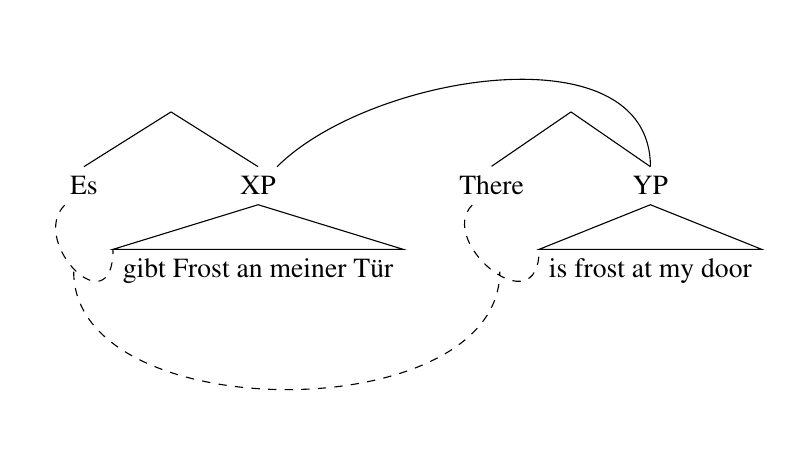
\begin{tikzpicture}
   \Tree [ [.\node(aDE){Es}; ]
    [.\node(pDE){XP};      
    \edge[roof]; \node(rDE){    gibt Frost an meiner Tür };  ] ] 
    \begin{scope}[shift={(2in,0in)}]
      \Tree [ [.\node(aEN){There};  ]
            [.\node(pEN){YP}; \edge[roof]; \node(rEN){ is frost at my door}; ] ]
          \end{scope}
          \draw[-] (pDE)..controls +(north east:2) and +(north:2) .. (pEN); 
          \draw[dashed,-] ($(rDE.west)-(0.5,0)$)..controls +(south:2) and +(south:2)..($(rEN.west)-(0.5,0)$); 
          \draw[dashed,-] (aEN)..controls +(south west:1) and +(south:1) .. (rEN.north west); 
          \draw[dashed,-] (aDE)..controls +(south west:1) and +(south:1) .. (rDE.north west); 
\end{tikzpicture}
   \caption{N-gram-samanstilling versus syntaktiske frasar}
    \label{fig:ikkjenode}
  \end{figure}

Men sett no at me ikkje har som formål å nytte frasesamanstillinga til
reint N-grambasert omsetjing. Kva for \emph{lingvistiske} krav kan me
stille til å kalle to frasar samanstilte? Me må i alle fall tillate
ein del skilnad.  I alle større parallelltekster vil parallellstilte
setningar ha visse syntaktiske og semantiske\footnote{Sidan eg går ut frå at data er setningssamanstilt, kjem eg
       ikkje inn på diskurs-/pragmatiske verknader, med mindre dette
       fører til forskjellar innanfor setningane (sjå t.d. del
       \ref{SEC:ordkrav} om lenkjer mellom koreferente substantiv og
       pronomen). } omsetjingsskifte,
t.d. leksikalisering av syntaktiske konstruksjonar eller omvendt,
endring av ordklasse, presisering/depresisering, endringar i leksikalske
trekk (t.d. telleleg/utelleleg),
osb. \citep[s.~56--62]{munday2001its}, slik at den einaste
fullstendige, «perfekte» samanstillinga vil vere
identitetsfunksjonen. Kor mykje mangel på samsvar me godtek blir då
avgjort av formålet med samanstillinga.

Eitt av formåla med samanstillinga i denne oppgåva er å kunne oppdage
korleis ulike språk realiserer semantiske roller syntaktisk; då
spesielt i forhold til hypotesane gitt i \citet[s.~7]{xpar2008rcn},
t.d. at «case marking might be useful to further determine a given
argument's semantic role». Skal me finne det siste, må me altså kunne
lenkje frasar med ulik kasusmarkering, men ha krav om lik tildeling av
semantiske roller; samtidig skal me sjå at me ikkje kan ha krav om lik
syntaktisk funksjon. I tillegg vil me sjølvsagt ikkje lenkje på tvers
av konstituentgrenser, sidan det er fullstendige konstituentar\footnote{LFG tillèt som nemnt diskontinuerlege konstituentar, men dette
        er ikkje det same som ikkje-konstituentar av typen «es gibt» /
        «there is». }
som fyller dei semantiske rollene.

Eit anna mogleg formål er å nytte desse frasesamanstillingane til
maskinomsetjing. \citet{riezler2006gmt} nyttar ein stokastisk
frasesamanstilling til å oppdage transfer-reglar for bruk i LFG-basert
generering i maskinomsetjing. Dette er reglar som omsett fragment av
ein f-struktur på kjeldespråket til f-strukturfragment på
målspråket. (Eit krav på utforminga av moglege transfer-reglar hindrar
at ein får reglar som lenkjar ikkje-konstituentar, eg kjem tilbake til
dette nedanfor.)  Samanstillinga utvikla her burde au kunne nyttast
til å finne slike transfer-reglar, men dette er ikkje noko eg har lagt
vekt på.

Nedanfor gir eg eit forslag til krav for frasesamanstilling, med desse
formåla i tankane. Om alle krava er moglege å implementere, er eit
separat problem.

\section{Frasesamanstilling i ein LFG-trebank}
\label{sec-3.3}


Samanstilte frasar bør ha nok semantisk likskap til å kunne opptre som
omsetjingar i liknande omgivnader
\citep[s.~74]{dyvik2009lmp}. \citet{thunes2003eal} gir nokre prinsipp
-- som er passande å ha som utgangspunkt -- for å fastslå det som kan
kallast \emph{omsetjingsmessig korrespondanse} (her for
ordsamanstilling). Dette er prinsipp som skal gjelde for eit litt
forskjellig formål, men som au «ligger nær opp til det vi intuitivt
mener er riktig» \citep[s.~2]{thunes2003eal}. Prinsippa blir nytta til
å lage ein gullstandard for ordsamanstilling\footnote{\cite[s.~2]{thunes2003eal}: «Våre prinsipper er satt
       opp for å tjene et bestemt formål, nemlig å samle inn data som
       metoden i Semantic Mirrors skal anvendes på», ein metode for å
       automatisk finne WordNet-liknande relasjonar frå
       parallelltekst. I denne metoden vil det vere naturleg med høge
       krav til presisjon, men kanskje lågare krav til dekning:
       speilmetoden skal finne leksikalske semantiske forhold som held
       på \emph{typenivå}, medan for trebanken er det viktigare korleis me
       kan annotere eit \emph{token} av t.d. eit verb i ein viss VP i ei
       gitt korpussetning. },
hovudsakleg for dei opne klassene, og er definert ved å vise til kva
for rolle eit argumentord speler, eller kva for rolletildeling eit
predikat eller modifiserande ord gir. Så for å t.d. samanstille to
verb må dei ha like mange semantiske argument (men argumenta treng
ikkje alle realiserast syntaktisk) og dei må \emph{tildele same roller};
medan argumenta må \emph{spele same rolle}, og både argument og adjunkt må
vere \emph{koreferente}. Lenkja ord må vere del av frasar som speler same
rolle i «det som er felles i interpretasjonene av [dei to setningane]»
\citep[s.~3]{thunes2003eal}.


Viss me tek utgangspunkt i det siste, vil det vere naturleg å i
tillegg lenkje desse frasane som speler same rolle i «det som er
felles i interpretasjonene».

Krava for ordsamanstillinga må au vere fylt for at desse frasane kan
samanstillast. Ei ordsamanstilling er altså naudsynt for ein
frasesamanstilling, og omvendt. Dette er berre problematisk om me
føreset at det eine er derivert av det andre; men dette har me ingen
\emph{a priori} grunn til å gjere. Krava eg her utviklar bør i staden
sjåast på som \emph{skrankar} på moglege samanstillingar i modellen (jamfør
\ref{SEC:omgrepsavklaring} om modellteoretiske grammatikkar), heller
enn derivasjonelle forhold. Samtidig er det som nemnt eit mål å finne
ut kor uavhengig me kan gjere oss av ordlenkjingsinformasjonen (dette
er au nyttig for implementasjonen), utan at det treng å gi krava ei
\emph{retning}.

Ei frasesamanstilling er ei skildring av forhold mellom \emph{fragment} av
setningar, dette er endå ein grunn til at det er naturleg å skildre
dei ønskelege forholda som skrankar på moglege samanstillingar. Me kan
setje skrankar på f-struktur-, konstituent- og ordsamanstilling
samtidig, utan å måtte ha krav om at den eine samanstillinga er
fullstendig (eller delvis) avleiia av den andre, før me veit om eit
slikt avleiingsforhold er empirisk fundert. Me kan i tillegg ha
ufullstendige samanstillingar i dei tilfella der det er ufullstendig
samsvar mellom setningane (der ei fullstendig samanstilling ville
brutt visse krav).

Sidan metoden er mynta på bruk i ein LFG-parsa trebank, og delvis vil
nytte denne annotasjonen som datagrunnlag, er det naturleg å nytte
same konsept som blir nytta i LFG\footnote{I tillegg finst andre positive biverknader av ein LFG-basert
       frasesamanstilling for bruk i denne samanhengen, som at ein kan
       studere kor parallelle dei parallelle grammatikkane i
       ParGram-prosjektet \citep{butt2002pgp} faktisk er, på ulike
       nivå (leksikon og argumentstruktur, c-struktur, f-struktur). } (f-struktur, c-struktur,
endosentrisitetsprinsipp, \xbar{}-tre, osb.)  au i desse krava til den
«beste» frasesamanstillinga; i den grad LFG gir ein generaliserbar
skildring av syntaks, bør desse krava vere generaliserbare til andre
teoriar, men ein del forhold som er avleidd av LFG-prinsipp må
sjølvsagt modifiserast om krava skal generaliserast til andre teoriar.

Utan skrankar i det heile vil alt kunne lenkjast til alt (noko som er
like unyttig som å ikkje lenkje noko); i del \ref{SEC:kandidatar} ser
eg på kva for typar element i dei lingvistiske analysane (ord,
grammatiske trekk, konstituentar, \ldots{}) det er fornuftig å tillate
lenkjer mellom. I avsnitta nedanfor spesifiserer eg kva som må til for
at me skal lenkje element av desse typane.

\section{Kva kan lenkjast?}
\label{sec-3.4}

\label{SEC:kandidatar}

Viss to uttrykk er samanstilt på setningsnivå (slik at me dimed kan gå
ut frå at dei er omsetjingar av kvarandre), og begge har ein
LFG-analyse, så har me iallfall tre ulike nivå kor me kan finne
ekvivalensforhold under setningsnivå:
\begin{enumerate}
\item mellom ord i setningane,
\item mellom f-strukturar,
\item mellom c-strukturnodar.
\end{enumerate}
På begge språk har me alle nivå -- det er ingen grunn til å lenkje på
tvers av nivå sidan forhold mellom desse nivåa er implisitt i
LFG-analysen.

Alle ord i setninga er \emph{kandidatar} for samanstilling med ord i
omsetjinga, men det kan godt hende at eit ord \emph{ikkje} har ei lenkje,
og me kan heller ikkje utelukke at det finst mange-til-mange-lenkjer
som ikkje kan «delast opp». Dette gjeld au nodane i c-strukturen.

Me utelukker lenkjing av ikkje-konstituentar som \emph{there is} på
c-strukturnivå sidan ei lenkje mellom to c-strukturnodar impliserer at
heile frasen under er lenkja. Det finst ingen c-strukturnodar som
dominerer berre \emph{there}, \emph{is} og ingen andre ord (heller ikkje \emph{es},
\emph{gibt}), så dette er ikkje lenkjekandidatar.  \emph{There is} og \emph{Es gibt}
i figur \ref{fig:ikkjenode} kan då ikkje samanstillast åleine, men
berre som del av ei ytre frasesamanstilling\footnote{Slike forhold kan me sjølvsagt finne igjen etter lenkjinga,
        men då vil me au kunne generalisere til andre ordformer. Eg
        kjem tilbake til dette i kapittel \ref{SEC:diskusjon}. }.

Når det gjeld f-strukturane er det ganske mange element me teoretisk
sett kunne ha lenkja, t.d. enkelttrekk som kasus eller dei uordna
mengdene med adjunkt, men det som er mest \emph{nyttig} og \emph{meiningsfullt}
er nok å berre lenkje der det er ei nær kopling til orda i
setninga. Sidan alle PRED-element i ein f-struktur unikt står for
predikerande ord, kan me -- gitt to samanstilte setningar -- la
\emph{kandidatane for samanstilling på f-strukturnivå} inkludere alle
desse PRED-elementa i f-strukturane til
setningane\footnote{I del \ref{SEC:fnord} kjem eg tilbake til spørsmålet om me vil
        inkludere visse f-strukturar utan PRED-element i kandidatane
        for samanstilling. }. PRED-element representerer semantiske bidrag som
oftast er påkrevde på begge språk i omsetjingar, medan andre
f-strukturtrekk gjerne er valfrie på det eine av språka; det er ikkje
alle språk som har t.d. obligatorisk kasusmarkering, og ein vil
kanskje nytte trebanken til å oppdage nettopp slik variasjon.
PRED-elementa er i tillegg gjerne enklare å knyte direkte opp mot den
konkrete, observerte tekststrengen (eventuelt testast mot korpora,
eller talarintuisjonar), medan t.d. eit trekk som aspekt kanskje er
umogleg å skilje frå tempus i affikset (det vil vere vanskelegare å
teste om ei lenkje mellom aspekt-trekk er empirisk motivert utan å dra
inn ein heil del teori).

Samtidig er det au eit omsetjingsforhold mellom trekka i same
f-struktur som dei lenkja PRED-elementa, og me ville kanskje ikkje ha
omsett dei to PRED-elementa i andre f-strukturkontekstar. Difor bør me
au sjå på ei PRED-lenkje som ei lenkje mellom \emph{f-strukturane til
desse PRED-elementa}\footnote{Eventuelt kunne me ha definert lenkjingskandidatane på
       f-strukturnivå som alle PRED-haldande f-strukturar, resultatet
       blir det same. }.  Med dette i tankane, kombinert med
c-struktur-f-strukturavbildinga $\phi$ (sjå del
\ref{SEC:omgrepsavklaring}), får me følgjande samanheng, illustrert i
figur \ref{fig:viss-PRED-så-f-og-c}:

\ex. \label{krav:f-links} Ei lenkje mellom to PRED-element $p$ og $q$, kor
      $p$ er medlem av f-strukturen $f$, og $q$ er medlem av
      f-strukturen $g$, tilseier at:
\a. \label{krav:f-links-substr} me tolkar f-strukturane $f$ og $g$ som lenkja,
\b. \label{krav:f-links-words} orda i setningane som projiserer
     PRED-elementa tek del i ei lenkje (kor andre
     ord kan vere involvert), og at
\c. \label{krav:f-links-domain} nodar innanfor $\phi^{-1}(f)$
     og $\phi^{-1}(g)$, dei funksjonelle domena til f-strukturane $f$
     og $g$, kan lenkjast

 \begin{figure}[htp]
    \centering
    \begin{tikzpicture}
    {\avmoptions{}
     \node(src){
        \begin{avm}
          $f$ \[pred  & `{\bf{}sove}<jeg>' \\
          tense & pret \\
          ... \]
        \end{avm}
      };
      \node[right of=src, node distance=5cm](trg){
        \begin{avm}
          $g$ \[pred   &  `{\bf{}sleep}<I>'\\
          tense  & pret  \\
          aspect & simple \\
          ... \]
        \end{avm}
      };
      }
      \draw[dashed,-] (src.west) .. controls +(-1,2) and +(-1,2) .. node[above,sloped]{$l_f$} (trg.west) ;
      \draw[-] ($(src.north)-(1,0.3)$) .. controls +(0,1.5) and +(0,1.5) .. node[above,sloped]{$l_p$} ($(trg.north)-(1,0.3)$) ;

      \begin{scope}[shift={(0,-3cm)}]
     \Tree  [.\node(VPs){VP}; [.\node(Vs){V}; \node(sov){sov};  ] ]
      \begin{scope}[shift={(5cm,0)}]
        \Tree  [.\node(VPt){VP}; [.\node(Vt){V}; \node(slept){slept};  ] ]
      \end{scope}
      \end{scope}
      \draw[-] (VPs)..controls +(north:1.5) and +(north:1.5) .. node[above,sloped]{$l_c$} (VPt) ;
      \draw[dashed,-] (sov)..controls +(north east:1.5) and +(north west:1.5) .. node[above,sloped]{$l_o$} (slept) ;
   \end{tikzpicture}
    
\fxnote{TODO: teikne inn f-domene}

    \caption{Ei PRED-lenkje $l_p$ kan tolkast som ei f-strukturlenkje
    $l_f$, og impliserer ei c-strukturlenkje $l_c$ mellom toppnodane i
    dei funksjonelle domena. Orda som projiserer PRED-elementa er med
    i ei lenkje $l_o$ (som kan inkludere fleire ord).}
   \label{fig:viss-PRED-så-f-og-c}
 \end{figure}

Punkt \ref{krav:f-links-substr} og \ref{krav:f-links-domain} over seier at viss
PRED-elementa projisert av t.d. to verb i verbfrasar er lenkja, kan
VP-ane som heilskap lenkjast, i tilfellet i figur
\ref{fig:viss-PRED-så-f-og-c} kan iallfall dei øvste nodane i VP-ane
lenkjast, i tillegg til f-strukturane frå ytre PRED til verba.  Det er
dette at heile VP-ane (kanskje inkludert objekt) er lenkja som gjer
det til ei fraselenkje og ikkje berre ei ordlenkje. Punkt
\ref{krav:f-links-substr} er forsvart over, medan punkt
\ref{krav:f-links-domain} kjem som ein konsekvens av at det er det
funksjonelle domenet som spesifiserer informasjonen i f-strukturane,
nodane her bør difor lenkjast berre viss f-strukturane er lenkja. Men
som punkt \ref{krav:f-links-domain} indikerer finst det au situasjonar der
nodar innanfor domena skal stå ulenkja.

Alle nodar i c-strukturen (alle syntaktiske \emph{frasar/konstituentar} i
setninga) som kan koplast til PRED-haldande f-strukturar, vil vere
kandidatar for samanstilling på c-strukturnivå (dette inkluderer
diskontinuerlege konstituentar), men ikkje alle vil bli lenkja.  I del
\ref{SEC:subnode} ser eg på kva som må til for å lenkje nodar i det
funksjonelle domenet.  I tillegg finst det nodar over ord som ikkje
projiserer PRED-element, desse kjem eg tilbake til i del
\ref{SEC:fnord}.

I følgje punkt \ref{krav:f-links-words} vil fraselenkja leie til at sjølve
verba i to lenkja VP-ar au er lenkja, som tilseier at \emph{ei PRED-lenkje impliserer ei ordlenkje}. I visse tilfelle er dette heilt
uproblematisk, t.d. viss \emph{I slept down by the river} skal lenkjast med
\emph{Eg sov nede med elva} vil me uansett lenkje \emph{slept} og \emph{sov}; dette
kan gjelde transitive verb au:

\ex. \a. The locusts have no king, just noise and hard language\\
     $\leftrightarrow$
     \b. Grashoppene har ingen konge, berre støy og krasse ord


\emph{have/har} tek del i VP-samanstillinga \emph{have no king.../har
ingen konge...}, her au skal det vere uproblematisk å lenkje
enkeltorda \emph{have} og \emph{har}.

Men som nemnd treng ikkje ordsamanstillinga vere ein-til-ein, det
punkt \ref{krav:f-links-words} seier er at desse orda iallfall er ein del
av ein samanstilling med kvarandre (i døme \Last altså
VP-samanstillinga). Kanskje er dette ei mange-til-mange-lenkje som
ikkje \emph{kan} reduserast til ein-til-ein-lenkjer; eller kanskje er
det som i \Last mogleg å skilje ut delsamanstillingar, som
\emph{have/har}. Eg kjem tilbake til dette
\fxnote[inline,nomargin]{TODO: når?} seinare.

Sidan PRED-lenkjing impliserer ordlenkjing, må me sjekke om krava på
ordnivå (del \ref{SEC:ordkrav}) er oppfylte for å lenkje to
PRED-element. \fxnote[inline,nomargin]{TODO: litt brå avslutning}

\section{Krav på ordnivå}
\label{sec-3.5}

\label{SEC:ordkrav}

Ord som skal lenkjast må i \cite{thunes2003eal} vere del av frasar som
speler same rolle i det som er felles i interpretasjonane, her kan me
omskrive det til at dei må vere del av \emph{frasar som er lenkja på c-strukturnivå}; forholda i \ref{krav:f-links} gir då koplinga til krav på
andre nivå (t.d. vil krav om tildeling av like mange roller vere
meir passande å spesifisere på f-strukturnivå).

Det er visse ting me ikkje kan spesifisere ut frå rein c- og
f-strukturinformasjon. Den norske setninga \emph{eg vil ete} kan fint
samanstillast med \emph{I want to eat}, med ei lenkje mellom \emph{ete} og
\emph{eat}. Men kva står i vegen for å lenkje \emph{ete} til hovudverbet i \emph{I want to drink}? Forskjellen på f-strukturnivå er berre at PRED-verdien
er ulik (\textbf{eat} mot \textbf{drink}). Me må altså ha eit krav om at tydinga til
lenkja ord (og deira predikat) er «lik nok» til at me kan sjå på dei
som omsetjingar\footnote{Eigentleg burde slike setningar ikkje vere lenkja på
        setningsnivå ein gong, men som me skal sjå i del
        \ref{SEC:lik-argstr} treng me kravet om lik tyding 
        sjølv innanfor setninga. }. \citet[s.~74]{dyvik2009lmp} krev at orda
generelt, utan kontekst, må vere semantisk plausible omsetjingar,
dvs. at målordet er eit medlem av mengda av \emph{linguistically predictable translations} av kjeldeordet. Målordet har då
\emph{LPT-korrespondanse} med kjeldeordet.  Nedanfor reknar eg
LPT-kravet som eit krav på ordnivå, og eg føreset at LPT-informasjonen
er ein type bottom-up-informasjon, som viser om to ord generelt (i
ulike kontekstar) blir nytta som omsetjingar av kvarandre. Denne
informasjonen kan reint praktisk komme frå automatisk
ordsamanstilling, eller ei god tospråkleg ordbok, det bør ikkje spele
nokon rolle for resten av krava\footnote{Ein kan au tenkje seg at ei djup semantisk dekomponering av
        kvart ord sto som grunnlag for LPT-informasjon -- men då vil
        LPT-korrespondanse mellom to ord implisere at orda er
        synonyme, heller enn generelt plausible omsetjingar. }.

\fxnote{TODO: Er det mogleg å presisere LPT-kravet meir? Skal det
berre vere eit rangeringskrav??}
 
Ein type presisering/depresisering (del \ref{SEC:formaal}) me ofte ser
i omsetjingar er at eit pronomen på kjeldespråket blir nytta der
målspråket har eit koreferent substantiv, eller
omvendt. \citet{dyvik2009lmp} opnar for at desse au har
LPT-korrespondanse (som nemnt i \cite{thunes2003eal} må lenkja ord
uansett vere koreferente).

Men kva då med lenkjing av pronomen til verb bøygd for person og tal i
pro-drop-språk?

\ex. \a. iqePa                                  \hfill{} (georgisk) \\
     $\leftrightarrow$
     \b. han bjeffa

Viss setningane i døme \Last er lenkja, der iqePa har eit pro-argument
koreferent med \emph{han} som subjekt, bør dei to subjekta iallfall kunne
lenkjast på f-strukturnivå; dei har same referent og speler same rolle
i argumentstrukturen til verba (som me går ut frå er lenkja). På
ordnivå, derimot, kan me ikkje lenkje \emph{han} til \emph{iqePa} åleine -- her
må me ha ei mange-til-ein-lenkje mellom $\{ \rm han, bjeffa \}$ og $\{
\rm iqePa \}$. 
Generelt må me ha slike lenkjer der eitt ord projiserer fleire
PRED-element\footnote{Me ville au fått ei mange-til-ein-lenkje om me tillot
        \emph{komplekse predikat} i analysane, t.d. slik
        \citet{butt1998merger} foreslår ved å la kombinasjonen av to
        ord endre argumentstrukturen til eitt PRED-element. }.

\subsection{Ordklasse}
\label{sec-3.5.1}

Ulike språk leksikaliserer same konsept på ulike
måtar. \citet[s.~3]{cheung2002scg} nemnar vanskane med å ha eit krav
om lik ordklasse i utviklinga av ein kinesisk-engelsk termbank, kor
t.d. det engelske ordet \emph{fulfilment} meir naturleg blir omsett til eit
verb på kinesisk. På same måte vil eit georgisk verbalsubstantiv
(\emph{masdar}) gjerne bli omsett til eit verb i infinitiv på
norsk. Slike skifte mellom ordklasser er svært vanlege i
omsetjing\footnote{\citet[Catford~(1965),~i][s.~61]{munday2001its} gir ein gjennomgang av
       slike \emph{klasseskifte}, og andre typar omsetjingsskifte. }.

Me kan opne for ordklasseoverskridande lenkjer der det er samsvar på
andre nivå, me bør iallfall krevje ein likskap i argumentstruktur; så
om LPT-kravet og krava på c- og f-strukturnivå er fylt, bør det ikkje
vere noko i vegen for å lenkje ord (eventuelt mengder av ord) av ulik
ordklasse.


\section{Krav på f-strukturnivå}
\label{sec-3.6}

\fxnote{problematiser: må me ha /PRED-lenkje/ frå arg til arg/adj? (ikkje
    krevd no...men skal me rangere ved det?)}
\fxnote{kryssande f-lenkjer?}
\fxnote{mange-mange-f-lenkjer?}
 
På f-strukturnivå har me direkte tilgang til informasjon om
argumentstrukturen til eit predikat, og mengda av adjunkt som
modifiserer predikatet. Når \citet[s.~3]{thunes2003eal} skriv at to
lenkja ord $a$ og $b$ må opptre i frasar som har «tilstrekkelig like
argumentstrukturer til at uttrykkene i \emph{a}s omgivelser står i de
samme semantiske relasjonene til hverandre og til \emph{a} som de
korresponderende uttrykkene i \emph{b}s omgivelser gjør til hverandre
og til \emph{b}» er det difor passande å prøve å gjere dette til eit
krav på f-strukturnivå.

Den enklaste lenkjingssituasjonen, f-strukturmessig, er der
rotpredikata kan lenkjast, og første argument av predikatet på
kjeldespråket kan lenkjast til første argument på målspråket, andre
argument til andre argument, osb., og lenkjinga kan fortsetje slik
rekursivt inn i f-strukturane. I ein slik situasjon er det fullstendig
samsvar mellom kor mange argument det finst på kvar side, og
fullstendig samsvar i det tematiske rollehierarkiet (dvs. kva for
posisjon kvar rolle har i argumentstrukturen), i heile strukturen.

Som me skal sjå er det ikkje vanskeleg å komme over situasjonar der
dette ikkje held, og me blir nøydt til å tillate lenkjer mellom
argument og adjunkt, og lenkjer som går på tvers av følgja i
argumentstrukturane. I tillegg kan me ikkje klare oss utan
LPT-informasjon for å avgjere \emph{når} me har å gjere med slike meir
komplekse situasjonar. 
\subsection{Krav om lik argumentstruktur}
\label{sec-3.6.1}

\label{SEC:lik-argstr}

\citet{thunes2003eal} gir som nemnd eit krav om at \emph{predikat må ha tilsvarande semantiske argument} for å lenkjast.

Om det alltid er slik at to predikat har like mange argument, som kjem i
same rekkjefølgje i argumentstrukturen, vil det gjere den praktiske
oppgåva med å lenkje predikata, og argument med argument, mykje
enklare. Men kan me stille så sterke krav?

Sett at ei setning på språk 1 har ei \emph{at}-setning som adjunkt, medan
denne setninga på språk 2 er eit argument, og at desse setningane
ville vore lenkja om dei opptredde åleine. Om dei uttrykkjer same
proposisjon og \emph{speler same rolle i verbsituasjonen}, synest det
naturleg å lenkje desse.

Slike omsetjingsrelasjonar gir data for verbsituasjonen, på eit meir
generelt grunnlag enn det me kan få frå einspråklege analysar
åleine. Om me har gode semantiske grunnar for å kalle ein deltakar i
ein verbsituasjon eit argument på eitt språk, vil dei same grunnane
gjelde for omsetjingsmessig korresponderande verb på andre språk. Ein
kan då nytte unionen over alle argument til korresponderande verb til
å karakterisere kva ein meiner med \emph{deltakarane i verbsituasjonen}. Syntaktiske forhold i språket kan sjølvsagt gi
grunnar til å \emph{ikkje} kalle dette eit argument.

For å gjere dette konkret kan me sjå på setning 7 i test-suiten til
XPar-prosjektet:

\exg.  abramsi brouns       daenajleva sigaretze, rom cvimda \\
      Abrams.NOM Brown.DAT vedde.3SG sigarett.om, at  regne.3SG.IMP \\
     `Abrams veddet en sigarett med Brown på at det regnet' 

I følgje LFG-parsen til desse setningane har hovudpredikata svært ulik
argumentstruktur\footnote{Analysane er henta 18. mai, 2009, frå
        \href{http://decentius.aksis.uib.no/logon/xle.xml}{http://decentius.aksis.uib.no/logon/xle.xml}, som implementerer
        LFG-grammatikkane frå ParGram-prosjektet \citep{butt2002pgp}. }. Det norske \emph{vedde} har \underline{fire} argument, medan
\emph{da-najleveba} har \underline{to} (\emph{Abrams} og \emph{Browne}), kor at-setninga på
norsk og \emph{rom cvimda} uttrykkjer same proposisjon og speler same rolle
i verbsituasjonen. Den engelske LFG-parsen av den tilsvarande setninga
(mine omsetjingar) gir \underline{tre} argument, \emph{with} blir her adjunkt, medan
den tyske grammatikken, som au har \underline{tre} argument, gjer \emph{at}-setninga
til adjunkt. I \Next nedanfor har eg representert dei omsetjingsmessig
korresponderande frasane i f-strukturane med dei norske omsetjingane
for å illustrere dette:

{\avmoptions{}
\ex. \label{ex:vedde}
\a. Adams veddet en sigarett med Browne \hfill{} (norsk bokmål)\\ på at det regnet.\\
    $\\\begin{avm}\[pred & `{\bf{}vedde}<Abrams, sigarett, Browne, regne>' \\
                 adjunct & \{\}\]\end{avm}\\$
\b. abramsi brouns daenajleva sigaretze, rom cvimda. \hfill{} (georgisk)\\
    $\\\begin{avm}\[pred &  `{\bf{}da-najleveba}<Abrams, Browne, regne>'\\
    adjunct &  \{ \rm sigarett \}\]\end{avm}\\$ 
\c. Abrams hat mit Browne um eine Zigarette gewettet, \hfill{}(tysk)\\
    daß es regnet.\\
    $\\\begin{avm}\[pred & `{\bf{}wetten}<Abrams, regne>' \\
                  adjunct & \{ \rm Browne, sigarett \}\]\end{avm}\\$
\d. Abrams bet a cigarette with Brown that it was raining. \hfill{}(engelsk)\\
    $\\\begin{avm}\[pred & `{\bf{}bet}<Abrams, sigarett, regne>'\\
                  adjunct & \{ \rm Browne \}\]\end{avm}$

}

Om ein skal ha grammatikkane som datagrunnlag er det altså eit reellt
problem kva ein skal gjere med mangel på samsvar i
argumentstruktur. Om det alltid var fullstendig samsvar i
argumentstruktur, ville det vore trivielt å lenkje argument: viss to
korresponderande verb hadde tre argument, ville me lenkja det første
med det første, det andre med det andre og det tredje med det
tredje. Men om me har analysar som dei over, ser det ut til at me er
avhengig av LPT-kravet frå del \ref{SEC:ordkrav} for å avgjere kva for
adjunkt og argument som samsvarer. 

LPT-kravet blir forresten endå viktigare når det gjeld lenkjing av
adjunkt til adjunkt. Adjunkt plukker ut si eiga rolle (argument får
rolla tildelt frå verbet) og f-strukturane ordnar ikkje adjunkt etter
nokon rekkjefølgje, dei er representert som uordna mengder, medan
følgja mellom argument iallfall potensielt kan nyttast til å indikere
semantisk likskap.

Ein kan argumentere for at grammatikkane her \emph{burde} hatt like (eller
likare) analysar, dette ville letta lenkjingsarbeidet, men sidan stoda
no er slik, må krava ta høgd for lenkjer mellom argument og
adjunkt. Om seinare utgåver av grammatikkane gir likare analysar, vil
det iallfall ikkje gi verre lenkjingsresultat.

Og ei enkel korpusundersøking tyder på at det er relativt sjeldan at
ein får slike situasjonar som \Last illustrerer.  I
\citet{unhammer2009aaa} analyserte eg setningane frå den manuelt
frasesamanstilte trebanken SMULTRON \citep{samuelsson2006pap} med
LFG-grammatikkane for engelsk og tysk i ParGram-prosjektet
\citep{butt2002pgp}, for å undersøkje følgjande hypotese:
\begin{quote}
participants in a verbal situation are expressed as
arguments (rather than adjuncts) in the source language of a
translation if and only if they are expressed as arguments (rather
than adjuncts) in the target language.
\end{quote}

Mellom anna fann eg at 2 av 15 korresponderande verbtoken hadde
LFG-analysar kor argument korresponderte med adjunkt\footnote{25 om ein inkluderer analysar kor minst eitt av argumenta
        ikkje hadde korrekt analyse (t.d. eit \textsc{PRO} der
        grammatikken burde funne eit substantiv). }. Her
utgjorde altså dei grammatiske analysane (ein del av) data, og
undersøkinga seier nok meir om analysane enn om språklege forhold. På
et så tynt datagrunnlag kan me vel berre konstatere at me må kunne
handtere argument-adjunkt-lenkjer når me prøver å lenkje, men
argument-argument-lenkjer bør prioriterast viss alt anna er likt.

\subsection{Ulik følgje i argumentstruktur}
\label{sec-3.6.2}

I tillegg til at argument kan lenkjast til adjunkt, kan koreferente
argument ha ulik følgje i argumentstrukturen. Det er klart at me vil
lenkje objektet til \emph{gefallen} (eller bokmål: \emph{behage}) med subjektet
til \emph{like}, og omvendt.  Men rekkjefølgje i argumentstrukturane i
ParGram-prosjektet er ofte basert på syntaktisk funksjon heller enn
rolle, slik at eit verb som har tema som subjekt og opplevar som
objekt vil ha tema før opplevar i argumentstrukturen, medan ei
omsetjing av dette verbet kan ha opplevar før tema:

{\avmoptions{}
\ex. \a. der Tonfall gefällt mir nicht \\
     $\begin{avm}\[pred & `{\bf{}gefallen}<Tonfall, ich$_i$>' ... \]\end{avm}$
    $\\\\\leftrightarrow$\\
     \b. jeg liker ikke tonen \\
     $\begin{avm}\[pred & `{\bf{}like}<jeg$_i$, tonen>' ... \]\end{avm}$

}

Argumentstrukturane i \Last har omvendt intern følgje. Igjen må me ha
LPT-informasjon for å avgjere kva for lenkjing som er korrekt. Men i
visse tilfelle vil ikkje ein gong LPT-informasjon vere nok:

{\avmoptions{}
\ex. \a. sie$_j$ gefallen ihnen$_i$ \\
     $\begin{avm}\[pred & `{\bf{}gefallen}<de$_j$, de$_i$>' \]\end{avm}$
    $\\\\\leftrightarrow$\\
     \b. de$_i$ liker dem$_j$ \\
     $\begin{avm}\[pred & `{\bf{}like}<de$_i$, de$_j$>' \]\end{avm}$

}

Det finst ingen f-strukturinformasjon eller LPT-informasjon me kunne
nytta til å sikre den korrekte lenkjinga \emph{sie/dem} og \emph{ihnen/de}; og
viss me rangerer lik argumentstruktur over ulik, vil me her få feil
resultat. Det me \emph{kan} gjere (utanom å endre grammatikkane slik at
argumentstruktur korresponderer med eit universelt tematisk
rollehierarki) er å sjå på mange lenkjingar av same verbpar, og på den
måten oppdage moglege feil. For enkelttilfelle, derimot, vil krava i
denne oppgåva ikkje vere nok til å gi korrekt lenkjing.


\subsection{Krav om argumentlenkjer}
\label{sec-3.6.3}

Sjølv om me ikkje krev lik følgje i argumentlenkjer, og tillèt
argument-adjunkt-lenkjer, er det eit minstekrav for å lenkje to
PRED-element at alle argumenta til det eine PRED-elementet kan
korrespondere med argument eller adjunkt av det andre PRED-elementet.
Dette følgjer av formålet med å finne ut korleis ulike språk
realiserer ulike semantiske roller syntaktisk; om eit verbargument
ikkje kan lenkjast til noko i omsetjinga (ikkje ein gong eit
pro-element), er det usannsynleg at verba uttrykker same situasjon, og
tildeler same roller. På same måte må sjølvsagt lenkja predikat ha
LPT-korrespondanse. \citet[s.~75]{dyvik2009lmp} gir følgjande krav på
f-strukturnivå:

\ex. \label{krav:PRED} Krav for lenkjing av to PRED-element $p$ og $q$:
\a. ordformene til $p$ og $q$ har LPT-korrespondanse
\b. alle argument av $p$ har LPT-korrespondanse med eit argument eller adjunkt av $q$
\c. alle argument av $q$ har LPT-korrespondanse med eit argument eller adjunkt av $p$
\d. LPT-korrespondansane er ein-til-ein
\e. ingen adjunkt til $p$ er lenkja til f-strukturar utanfor $q$, og omvendt

Det \Last[d] seier er at me ikkje lenkjer t.d. to instansar av «hest»
på det eine språket til éin instans av «horse» på det andre. Krav
\Last[e] kjem eg tilbake til nedanfor.

Det går an å gjere \Last strengare, og krevje at argumenta -- i
tillegg til å ha LPT-korrespondanse -- sjølv er PRED-lenkja. Dette har
eg ikkje gjort i implementasjonen min, men det er mogleg å ha det som
eit rangeringskriterium, noko eg kjem tilbake til i del
\ref{SEC:rangering}. Ved å \emph{ikkje} krevje at lenkjinga går heilt til
botn i f-strukturen blir det mogleg å seie at \emph{setningane} er
syntaktisk like, og at kanskje visse overordna frasar er syntaktisk
like, men visse \emph{delfrasar} kan likevel vere ulike og dimed ikkje vere
lenkja.

Kva med f-strukturomgivnadene til $p$ og $q$, skal me krevje at dei er
like?  I \Last[e] har me eit krav om at adjunkt til $p$ ikkje er
lenkja til f-strukturar utanfor $q$, og omvendt. Men viss $a_p$ er eit
adjunkt til $p$, kan det lenkjast til ein \emph{dotternode} av argument
eller adjunkt til $q$? La $a_q$ vere eit argument eller adjunkt til
$q$, viss $a_q$ er eit argument må det ved \Last ha LPT-korrespondanse
med argument/adjunkt i $p$, men det treng ikkje vere lenkja -- viss
det er ulenkja gjeld ikkje krav \Last for $a_q$, så \Last hindrar
ikkje ei lenkje mellom $a_p$ og døtre av $a_q$. 

I tillegg vil ikkje \Last hindre at t.d. den ytste f-strukturen i
kjeldespråket er lenkja til eit XCOMP-argument på målspråket; men i
dette tilfellet bør kanskje ikkje \emph{setningane} vere lenkja i
utgangspunktet.

Sjølv om det er logisk mogleg å gjere slike lenkjingar, er det
vanskeleg å finne ikkje-vilkårlege avgrensingar for når ein skal kunne
lenkje f-strukturar som står i ulike omgivnader; i implementasjonen
min har eg difor følgt eit strengare krav enn \Last[e]:

\ex. \label{krav:PRED-omgivnad} PRED-elementa $p$ og $q$ kan berre
     lenkjast om dei er ytste f-strukturar i lenkja setningar, eller
     er argument/adjunkt til lenkja f-strukturar.

Dette er ei tentativ formulering. Til no har eg ikkje sett døme kor
\Last ikkje bør gjelde, men om det finst slike døme bør sjølvsagt
kravet modifiserast.

Krav \ref{krav:PRED} og \ref{krav:PRED-omgivnad} bør i enkle
situasjonar vere tilstrekkelege for lenkjing på f-strukturnivå, men
det finst au meir komplekse korrespondansar mellom PRED-element. Desse
ser eg på del \ref{SEC:f-mange-mange}.

\subsection{\textbf{SKRIV} Adposisjonsobjekt}
\label{sec-3.6.4}


I følgjande setningspar har me eit objekt «sigarett» som svarer til
PP-en «sigaretze» («sigareti» + «ze»), eit adjunkt:

\begin{verbatim}
 Abrams veddet en sigarett med Browne på at det regnet.
 abramsi brouns daenajleva sigaretze, rom cvimda.
\end{verbatim}


\begin{verbatim}
 F_s [ PRED sigarett ]
\end{verbatim}


\begin{verbatim}
 F_t [ PRED ze<1> 1[ PRED sigareti ] ]
\end{verbatim}


F$_s$ og F$_t$ er døtre av dei ytre predikata i kvar setning, krav (iii)
seier at det må vere LPT-korrespondanse mellom desse for at me skal
kunne lenkje «veddet» og «daenajleva».  Her synest det feil å føye
saman «sigareti» og «ze», \texttt{(F\_s . (F\_t 1))}, sidan «sigarett» ikkje
inneheld informasjonen gitt av «ze».

Det finst då to løysingar. Me kan slakke på LMT-kravet ved å la
\texttt{L'(F\_t) = \{sigaretze, ze\}} (evt. \texttt{\{sigaret, ze\}}), då kan me lenkje
\texttt{(F\_s . F\_t)}, medan 1 er ulenkja.

Eller me kan lenkje \texttt{(F\_s . 1)}, kor me har skikkeleg
LMT-korrespondanse, men då må me slakke på (iii) og (iv), og altså ha
lov til å «hoppe over» ein f-struktur for å lenkje «veddet» og
«daenajleva». F$_t$ er då ulenkja. Det er løysinga valt i
\citet[s.~75,~fotnote~3]{dyvik2009lmp}, og den løysinga eg følgjer
vidare i oppgåva.

\subsection{\textbf{SKRIV} Kausativar og inkorporering}
\label{sec-3.6.5}

\label{SEC:f-mange-mange}
Til no har me føresett at eit PRED-element anten er ulenkja, eller
er lenkja til eitt og berre eitt anna PRED-element. Men i visse
tilfelle kan det vere ønskeleg å lenkje til fleire PRED-element.
\fxnote{Denne delen treng fleire ekte døme, og forsvar for kvifor me
vil ha ein-mange-lenkjer for våre \emph{formål} (georgisk ser ut til å vere
borte frå xle-web?)}

I ein norsk \emph{la}-konstruksjon, t.d. den me har i «å la noko fryse» (i
tydinga å forårsake at noko frys til) har me semantiske bidrag frå
både \emph{la} og hovudverbet \emph{fryse}, og begge har PRED-element (sjølv om
bidraget frå \emph{la} nok er meir «grammatisk»). Men slike perifrastiske
kan gjerne omsetjast til leksikaliserte kausativar som berre har eitt
PRED-element, men likevel med tydinga «å la fryse». Påfunnet i
\Next illustrerer denne situasjonen:

{\avmoptions{}
\ex. \a. ho lar-fryse huset \\
     $\begin{avm}\[pred & `{\bf{}la-fryse}<ho, hus>' \]\end{avm}$
     $\\\\\leftrightarrow$\\
     \b. ho lar huset fryse \\
     $\begin{avm}\[pred & `{\bf{}la}<ho, hus, XCOMP>' \\
     xcomp & \[pred & `{\bf{}fryse}<hus>'\]\]\end{avm}$

}

Her er altså den kausative tydinga leksikalisert, og verbet har berre
eitt PRED-element (på same måte som det norske verbet \emph{kjøle} berre
har eitt PRED-element, ikkje \emph{la} + \emph{bli kald}).\footnote{Det går sjølvsagt an å analysere sjølv leksikaliserte
        kausativar som om dei har fleire PRED-element, men det bør i
        såfall skje på uavhengig grunnlag, ikkje for å gjere lenkjinga
        enklare. }

Den same situasjonen får me der eit argument eller adjunkt er
inkorporert i verbet på det eine språket, men uttrykt som eit separat
predikat på det andre språket, t.d. samisk \emph{fierpmástallat} som på
norsk blir \emph{å fiske med garn} -- to predikat på norsk tilsvarer eitt
på samisk.

I \Last har \emph{la-fryse} to argument, som ved krav \ref{krav:PRED} begge
må finne korresponderande argument eller adjunkt for å lenkje \emph{la-fryse}. 
Då går det ikkje an å lenkje \emph{la-fryse} til berre \emph{fryse},
som har eitt argument; me får eit XCOMP til overs som manglar
lenkje. Me kan heller ikkje lenkje berre \emph{la} til \emph{la-fryse}, sidan
det då får ein XCOMP til overs.

Men, ved å ha ei ein-mange-lenkje, frå \emph{la-fryse} til både \emph{la} og \emph{fryse},
kan me oppfylle krav \ref{krav:PRED}. Då treng ikkje
XCOMP-argumentet lenkjast til eit argument av \emph{la-fryse}, det er
allereie lenkja til PRED-elementet; det som står igjen er unionen av
argumenta til \emph{la} og \emph{fryse}, desse må alle ha LPT-korrespondanse med
argument eller adjunkt av \emph{la-fryse}, og omvendt må alle argument av \emph{la-fryse} 
ha LPT-korrespondanse med argument eller adjunkt av \emph{la}
eller \emph{fryse} (utanom XCOMP-argumentet til \emph{la}, som allereie har ei
lenkje). Ein kan tolke dette som om \emph{la} og \emph{fryse} var samanføyd til
eitt predikat som krevde to argument (her: \emph{ho} og \emph{huset}).

Den einaste formelle forskjellen mellom dette og
substantivinkorporering blir då at substantivet ikkje krev eigne
argument. Det er au mogleg å tenkje seg ein kausativ med eit
inkorporert objekt, omsett til \emph{la + hovudverb + objekt}, altså ei
lenkje frå eitt PRED til tre PRED. Igjen vil me då sjå på dei resterande
ulenkja argumenta på kvar side; kvar av desse må lenkjast med eit
unikt argument eller adjunkt.

Men det bør kanskje vere grenser for kor langt slik samanføying kan
gå, om ikkje anna fordi problemet fort blir komputasjonelt
vanskeleg. Å opne for ein-mange-lenkjer mellom PRED-element (eller til
og med mange-mange-lenkjer) gir ei mykje større mengd moglege
løysingar på lenkjingsproblemet; i alle situasjonar der me krev
LPT-korrespondanse mellom eit argument $a_p$ av $p$ og eit adjunkt
$a_q$ av $q$ for å lenkje $p$ og $q$, vil me no au ha ei mogleg
løysing der $a_q$ er ulenkja, medan $a_p$ er samanføyd med $p$ og
difor ikkje treng LPT-korrespondanse med argument/adjunkt av $q$. Så
kan det au hende at $a_p$ sjølv kan samanføyast med eit av sine
argument/adjunkt. Skal me sjå etter slike løysingar samtidig som me
ser etter løysingar med ein-ein-lenkjer, vil me måtte leite gjennom
mange ufruktbare stiar. Ein måte å unngå dette på er å nedprioritere
samanføying, og berre prøve dette der det ikkje finst andre
alternativ.

Men det er ikkje berre av omsyn til implementasjonen ein bør
nedprioritere desse. Ei ein-mange-lenkje tyder på ein type
omsetjingsskifte, og det er ønskeleg å først sjå etter samanstillingar
som føreset syntaktisk likskap, før ein ser etter
omsetjingsskifte. Den viktigaste informasjonen me har å gå på er at
setningane er omsetjingar og difor har ein viss likskap -- Ockhams
barberkniv gir oss då grunn til å velje ei løysing som føreset lik
syntaks over ei løysing som føreset ulik syntaks. Viss det er mogleg å
opprette ei samanstilling på bakgrunn av lik syntaks, vil me
prioritere denne.

I implementasjonen blir difor alle ein-til-ein-lenkjer prøvd
først. \fxnote[inline,nomargin]{TODO:implementere:} Sidan kan ein
prøve å føye saman eit ulenkja PRED-element $p$ med eit ulenkja
PRED-element $a_p$ kor $a_p$ er argument eller adjunkt av $p$, og der
$p$ og $a_p$ vil kunne lenkjast med eit ulenkja PRED-element $q$ ved
føringane gitt over, og alle dei andre lenkjingskrava er dekkja. Me
får då eit modifisert krav \ref{krav:PRED}:

\ex. \label{krav:f-ein-mange} Krav for samanføyd lenkjing frå PRED-elementa
$p$ og $a_p$, kor $a_p$ er eit argument eller adjunkt av $p$, til PRED-elementet $q$:
\a. ordformene til $p$ og $a_p$ har saman LPT-korrespondanse med ordformen til $q$
\b. la $A$ vere unionen av argument til $p$ og argument til $a_p$,
    utanom $a_p$ sjølv;
    alle element av $A$ har LPT-korrespondanse med eit argument eller adjunkt av $q$
\c. la $D$ vere unionen av argument eller adjunkt til $p$ og argument
    eller adjunkt til $a_p$, utanom $a_p$ sjølv;
    alle argument av $q$ har LPT-korrespondanse med eit element av $D$
\d. LPT-korrespondansane er ein-til-ein
\e. ingen adjunkt til $p$ eller $a_p$ er lenkja til f-strukturar utanfor $q$, og ingen
    adjunkt til $q$ er lenkja til f-strukturar utanfor $p$

Det er trivielt å utvide dette kravet til å fungere for
mange-mange-lenkjer au.
\section{Krav på c-strukturnivå}
\label{sec-3.7}

\label{SEC:subnode}

Ein f-struktur er projisert av ei mengd c-strukturnodar, det vil seie
at det er desse nodane -- det funksjonelle domenet til f-strukturen --
som spesifiserer informasjonen som står i f-strukturen. Viss me har
grunnlag for å lenkje to f-strukturar, vil me au ha grunnlag for å
lenkje nodane som projiserte desse f-strukturane. Og omvendt vil det
aldri vere grunnlag for å ha ei c-strukturlenkje som står i konflikt
med f-strukturlenkjer, dvs. kor $\phi$ av kjeldenoden er lenkja til
noko anna enn $\phi$ av målnoden (då burde kjeldenoden vore lenkja til
dette andre). Det at to nodar er lenkja på c-strukturnivå må i det
minste implisere at informasjonen dei projiserer korresponderer. I
utgangspunktet bør krevje følgjande:

\ex.\label{krav:subnode-f-lenkja} to c-strukturnodar $n_s$ og $n_t$ kan
     berre lenkjast om $\phi(n_s)$ og $\phi(n_t)$ er lenkja på
     f-strukturnivå

Det enklaste ville vere å berre seie at alle nodane i dei to
funksjonelle domena er mange-mange-lenkja med kvarandre, men denne
lenkja vil ikkje gi oss meir informasjon enn at sjølve f-strukturane
er lenkja; ei lenkje på c-strukturnivå bør kunne gi meir nyansert
informasjon.

Det viktige forholdet på c-strukturnivå er \emph{dominans}; hovudgrunnen
til at me snakkar om c-struktur er at me vil skildre den hierarkiske
inndelinga av frasestrukturen i setninga, der ein node på høgare nivå
\emph{dominerer} mengder av nodar på lågare nivå. Ei lenkje mellom to
c-strukturnodar må altså implisere at det dominerte materialet
korresponderer.


\begin{figure}[htp]
\centering
  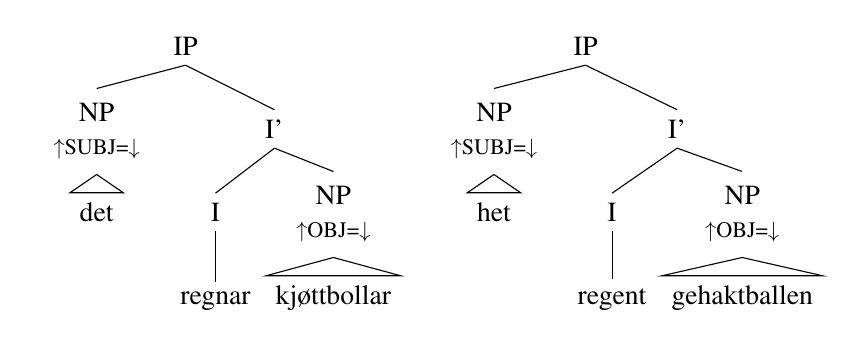
\begin{tikzpicture}
  \Tree  [.\node(IPs){IP};  [.\node(SUBJs){\proj{NP}{\ua SUBJ=\da}}; \edge[roof]; {det} ]
                            [.\node(I's){I'};
                                    [.\node(Is){I}; {regnar} ]
                                    [.\node(OBJs){\proj{NP}{\ua OBJ=\da}}; \edge[roof]; {kjøttbollar} ] ] ]
      \begin{scope}[shift={(2in,0in)}]
  \Tree  [.\node(IPt){IP};  [.\node(SUBJt){\proj{NP}{\ua SUBJ=\da}}; \edge[roof]; {het} ] 
                            [.\node(I't){I'}; 
                                    [.\node(It){I}; {regent} ]
                                    [.\node(OBJt){\proj{NP}{\ua OBJ=\da}}; \edge[roof]; {gehaktballen} ] ]   ]
\end{scope}
\end{tikzpicture}
   \caption{Enkel lenkjing av c-strukturnodar mellom norsk og
   nederlandsk; IP til IP, I' til I' og I til I.}
   \label{fig:enkel-c-lenkje}
  \end{figure}

I figur \ref{fig:enkel-c-lenkje} er dei funksjonelle domena til \emph{regnar/regent} 
lenkja\footnote{I desse trea har eg annotert f-strukturforhold på visse nodar;
       der eg ikkje har teikna inn dette gjeld $\ua=\da$, altså at
       noden er i same funksjonelle domene som mornoden. Eg har i
       tillegg forenkla kategorinamna ein del frå dei som kjem direkte
       frå ParGram/XPar-analysane, det bør ikkje ha noko å seie for
       framstillinga her. }, og det same med \emph{det/het} og \emph{kjøttbollar/gehaktballen}. 
Viss me føreset at subjekt-NP-ane er lenkja med kvarandre, og at
objekt-NP-ane er lenkja med kvarandre, på c-strukturnivå,
vil det vere ønskeleg å ein-ein-lenkje IP-nodane, I'-nodane og
I-nodane. Me skal sjå kvifor.

IP-nodane bør lenkjast sidan dei dominerer alt innanfor dei
lenkja funksjonelle domena; det finst ikkje ein gong nodar som står
utanfor det dei dominerer. Dei nodane som står nedanfor det funksjonelle
domenet til IP-ane er i tillegg lenkja med kvarandre. Det vil seie at
det ikkje finst informasjon på kjeldespråket som ikkje er uttrykt på
målspråket (eller omvendt) innanfor det IP-ane dominerer.

I'-nodane dominerer ikkje subjekta i figur
\ref{fig:enkel-c-lenkje}. Ei lenkjing av I'-nodane impliserer at det
som står under desse korresponderer, men au at nodane står i liknande
omgivnader. Det er lett å sjå føre seg eit døme der det ikkje ville
vore ønskeleg med ei lenkje mellom I'-nodane. I figur
\ref{fig:ikkje-c-lenkje} vil me t.d. ikkje lenkje desse nodane, på
norsk dominerer I' subjektet, som er lenkja til subjektet på
nederlandsk, men på nederlandsk står ikkje subjektet under I', og omvendt for
objektet. Ei lenkje mellom I'-nodane ville sagt at nodane dei
dominerte projiserte korresponderande informasjon, det gjer dei ikkje
i figur \ref{fig:ikkje-c-lenkje}. (I \ref{fig:enkel-c-lenkje}, derimot,
står dei lenkja objekta under I', medan dei lenkja subjekta er
utanfor.) Men merk at IP-nodane likevel kan lenkjast, dei dominerer
begge både subjekt og objekt, sjølv om dei kjem i ulik følgje under.
I-nodane dominerer berre verba, og kan au lenkjast.

\begin{figure}[htp]
\centering
  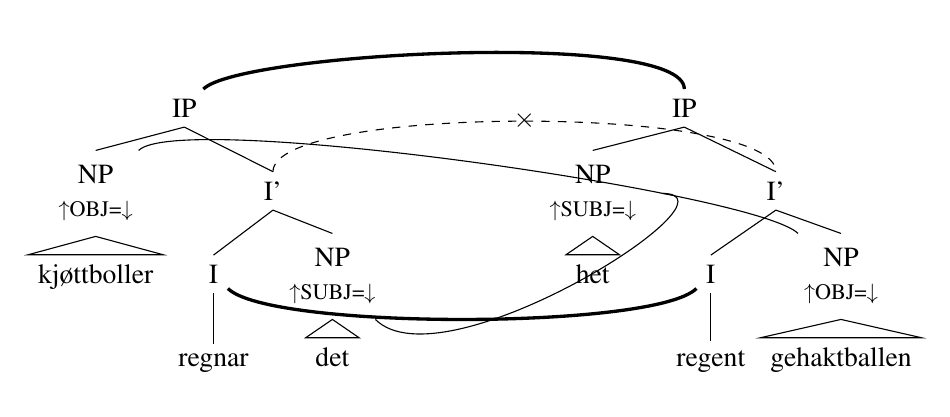
\begin{tikzpicture}
  \Tree  [.\node(IPs){IP};  [.\node(OBJs){\proj{NP}{\ua OBJ=\da}}; \edge[roof]; {kjøttboller} ]
                            [.\node(I's){I'};
                                    [.\node(Is){I}; {regnar} ]
                                    [.\node(SUBJs){\proj{NP}{\ua SUBJ=\da}}; \edge[roof]; {det} ]
                                     ] ]
      \begin{scope}[shift={(2.5in,0in)}]
  \Tree  [.\node(IPt){IP};  [.\node(SUBJt){\proj{NP}{\ua SUBJ=\da}}; \edge[roof]; {het} ] 
                            [.\node(I't){I'}; 
                                    [.\node(It){I}; {regent} ]
                                    [.\node(OBJt){\proj{NP}{\ua OBJ=\da}}; \edge[roof]; {gehaktballen} ] ]   ]
\end{scope}
\draw[-,very thick] (IPs)..controls +(north east:1) and +(north:1) .. (IPt) ;
\draw[dashed,-] (I's)..controls +(north:1.1) and +(north:1.1) .. node[midway,sloped]{$\times$} (I't) ;
\draw[-] (SUBJs)..controls +(south east:2) and +(east:2) ..  (SUBJt) ;
\draw[-] (OBJs)..controls +(north east:1.5) and +(north west:1.5) ..  (OBJt) ;
\draw[-,very thick] (Is)..controls +(south east:1) and +(south west:1) ..  (It) ;

\end{tikzpicture}
   \caption{C-strukturlenkjer kan ikkje gå på tvers av dominerte
   lenkjer (nynorsk og nederlandsk)}
   \label{fig:ikkje-c-lenkje}
  \end{figure}

Sjølv om subjektet sto ulenkja, t.d. ved lenkjing inn i eit
pro-drop-språk eller liknande, ville me fått same situasjon; I'-nodane
i figur \ref{fig:ikkje-c-lenkje-pro-drop} kan ikkje lenkjast sidan I'
på islandsk dominerer objektet, medan I' på norsk ikkje gjer dette, og
objekta er lenkja med kvarandre (her både på c- og f-strukturnivå). Ei
lenkje mellom desse I'-nodane ville sagt at dei dominerer
korresponderande materiale, men det gjer dei ikkje.

  \begin{figure}[htp]
  \centering
    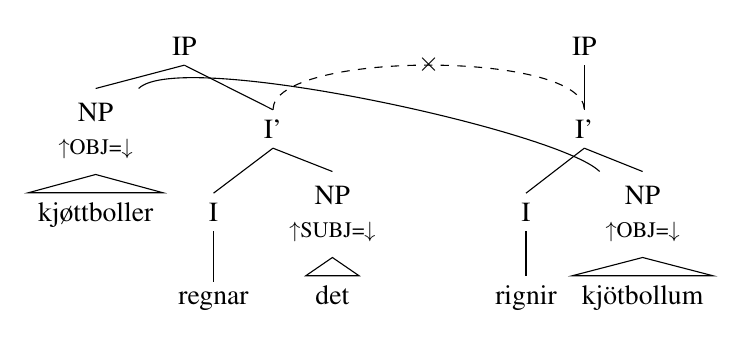
\begin{tikzpicture}
    \Tree  [.\node(IPs){IP};  [.\node(OBJs){\proj{NP}{\ua OBJ=\da}}; \edge[roof]; {kjøttboller} ]
                              [.\node(I's){I'};
                                      [.\node(Is){I}; {regnar} ]
                                      [.\node(SUBJs){\proj{NP}{\ua SUBJ=\da}}; \edge[roof]; {det} ]
                                       ] ]
        \begin{scope}[shift={(2in,0in)}]
    \Tree  [.\node(IPt){IP};  
                              [.\node(I't){I'}; 
                                      [.\node(It){I}; {rignir} ]
                                      [.\node(OBJt){\proj{NP}{\ua OBJ=\da}}; \edge[roof]; {kjötbollum} ] ]   ]
  \end{scope}
\draw[dashed,-] (I's)..controls +(north:1) and +(north:1) .. node[midway,sloped]{$\times$} (I't) ;
\draw[-] (OBJs)..controls +(north east:1.5) and +(north west:1.5) ..  (OBJt) ;
  
  \end{tikzpicture}
     \caption{C-strukturlenkjer kan ikkje gå på tvers av dominerte
     lenkjer (nynorsk og islandsk)}
     \label{fig:ikkje-c-lenkje-pro-drop}
    \end{figure}


Når treet deler seg i to som i desse figurane, får me ei mogleg
oppdeling av kjeldene til f-strukturinformasjonen. Me vil ikkje lenkje
nodar som ikkje gir same tilskot til f-strukturen, på same måte som me
ikkje vil lenkje på tvers av f-strukturlenkjer.

I både figur \ref{fig:ikkje-c-lenkje} og figur
\ref{fig:ikkje-c-lenkje-pro-drop} er det slik at det I'-nodane dominerer gir
ulike tilskot til f-strukturen, dei kan difor ikkje lenkjast. Likevel
må me tillate litt slingringsmonn her, nodane skal ikkje trenge
projisere heilt like f-strukturar. Det som er relevant er det som blir
lenkja i f-strukturen.

Som desse døma viser må me nyansere prinsippet om å ikkje lenkje
c-strukturnodar på tvers av f-strukturlenkjer, til å ta innover
seg dominans: me vil ikkje lenkje c-strukturnodar viss \emph{det dei dominerer} kjem i konflikt med f-strukturlenkjer.


I visse tilfelle kan det hende at sjølv toppnodane i det funksjonelle
domenet ikkje bør lenkjast. I døma over dominerer toppnoden i det
funksjonelle domenet, IP, alt som står under $\phi(IP)$ i
f-strukturen.  I figur \ref{fig:ikkje-c-lenkje-toppnode}, derimot, er
objektet til \emph{regna} ikkje dominert av toppnoden i det funksjonelle
domenet til \emph{regna}, VP-en; men det er lenkja til objektet i
funksjonelle domenet til \emph{rained}. F-strukturane til dei to VP-ane er
lenkja, men toppnodane i dei funksjonelle domena kan ikkje lenkjast
sidan dei to toppnodane dominerer materiale som inneheld ulike lenkjer
på f-strukturnivå -- ei slik c-strukturlenkje ville stått i konflikt
med f-strukturlenkjene. Intuitivt synest det au feil med ei lenkje
mellom konstituentane \emph{det regner} og \emph{it rained meatballs}. Dei kan
iallfall ikkje reknast som omsetjingar av kvarandre åleine; i ein
større kontekst kan dei inngå i ein korrespondanse, men denne større
konteksten har me jo lenkja allereie ved IP-nodane.

  \begin{figure}[htp]
  \centering
    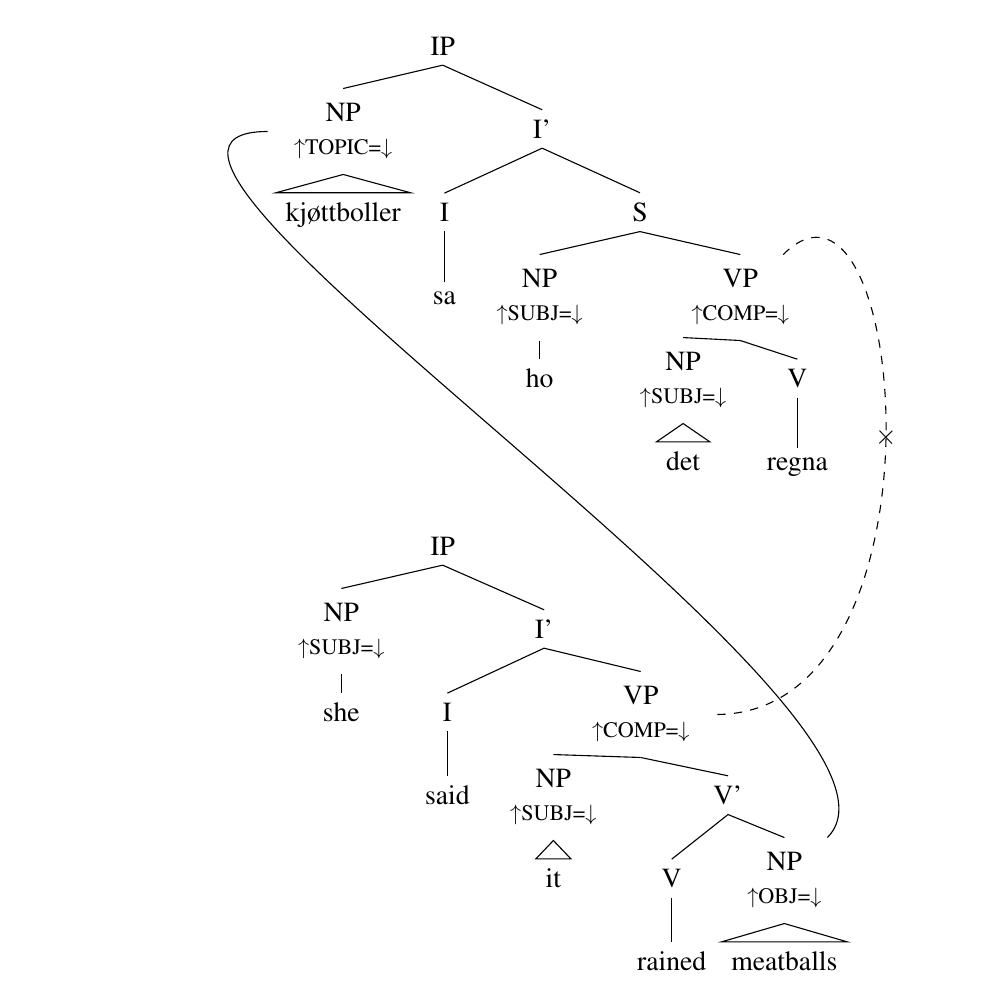
\begin{tikzpicture}
     \Tree  [.\node(IPs){IP};  [.\node(OBJs){\proj{NP}{\ua TOPIC=\da}}; \edge[roof]; {kjøttboller} ]
                               [.\node(I's){I'};
                                       [.\node(Is){I}; {sa} ]
                                       [.\node(Ss){S};
                                               [.\node(SPKRs){\proj{NP}{\ua SUBJ=\da}}; {ho} ]
                                               [.\node(VPs){\proj{VP}{\ua COMP=\da}}; [.\node(SUBJs){\proj{NP}{\ua SUBJ=\da}}; \edge[roof]; {det} ]
                                                                                      [.\node(Vs){V}; {regna} ] ] ] ] ]
         \begin{scope}[shift={(0in,-2.5in)}]
    \Tree  [.\node(IPs){IP};  [.\node(SPKRt){\proj{NP}{\ua SUBJ=\da}}; {she} ]
                               [.\node(I's){I'};
                                       [.\node(It){I}; {said} ]
                                       [.\node(VPt){\proj{VP}{\ua COMP=\da}}; [.\node(SUBJt){\proj{NP}{\ua SUBJ=\da}}; \edge[roof]; {it} ]
                                                                              [.\node(V't){V'}; [.\node(Vt){V}; {rained} ]
                                                                                                [.\node(OBJt){\proj{NP}{\ua OBJ=\da}}; \edge[roof]; {meatballs} ]
 ] ] ] ]
  \end{scope}
  %\draw[-] (SPKRs)..controls +(south west:3) and +(west:3) ..  (SPKRt) ;
  \draw[dashed,-] (VPs)..controls +(north east:3) and +(east:4) ..  node[midway,sloped]{$\times$} (VPt) ;
  \draw[-] (OBJs)..controls +(west:4) and +(north east:3) ..  (OBJt) ;
  
  \end{tikzpicture}
     \caption{Sjølv toppnodane i eit funksjonelt domene kan stå
     ulenkja; her kan ikkje VP-nodane lenkjast sidan det norske
     \TOPIC{} er objektet til \emph{regna}, lenkja til objektet under
     VP på engelsk}
     \label{fig:ikkje-c-lenkje-toppnode}
    \end{figure}

I det minste bør me difor krevje følgjande av lenkjer på c-strukturnivå:
\ex.\label{krav:c-tentativt} Ein node $n_s$ kan lenkjast med ein node $n_t$ berre viss:
\a. $\phi(n_s)$ er lenkja på f-strukturnivå med $\phi(n_t)$, og
\b. det ikkje finst nodar under $n_s$ som er lenkja med nodar utanfor det funksjonelle domenet
    til $n_t$, og 
\c. det ikkje finst nodar under $n_t$ som er lenkja med nodar utanfor det funksjonelle domenet
    til $n_t$.

Men, kva om det finst nodar under $n_s$ som ikkje er lenkja på
c-strukturnivå (kanskje fordi det ikkje finst tilsvarande nodar på
målspråket, t.d. ved lenkjing inn i pro-drop-språk), men som har ei
lenkje på f-strukturnivå?  Her finst det fleire alternative løysingar,
som eg ser på nedanfor.

\subsection{Lenkja f-strukturar utan c-strukturnodar}
\label{sec-3.7.1}

\label{SEC:f-lenkje-utan-c-node}

I figur \ref{fig:gaiGo} kan iallfall IP-nodane lenkjast, dei dominerer
alle orda på begge setningane, og f-strukturane er lenkja. Men
NP-subjektet på den norske sida, er ikkje lenkja med noko i det
georgiske treet; dette subjektet er lenkja med eit pro-element på
f-strukturnivå. Den informasjonen (her reint syntaktisk) som ordet
\emph{det} tilfører IP, ligg under I' på georgisk. Ved I-nodane manglar
det norske treet i tillegg den informasjonen som \emph{seg} tilfører.

\begin{figure}[htp]
\centering
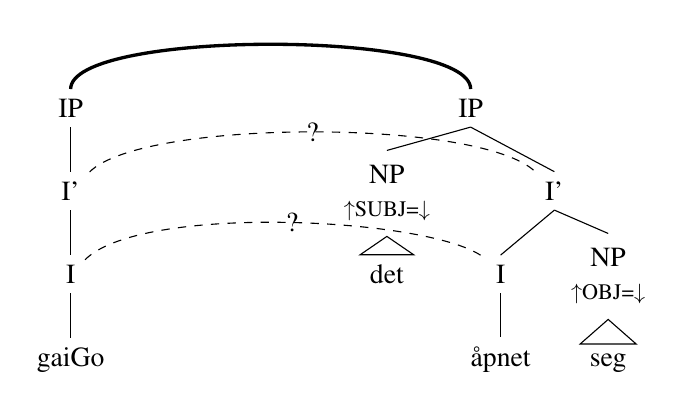
\begin{tikzpicture}
\Tree [.\node(IPk){IP}; 
  [.\node(Ibark){I'};  [. \node(Ik){I};  \node(gaiGo){gaiGo};  ]
  ] ]
     \begin{scope}[shift={(2in,0in)}]
\Tree [.\node(IPb){IP}; 
  [.\proj{NP}{\ua SUBJ=\da} \edge[roof]; {det} ] 
  [.\node(Ibarb){I'};  [.\node(Ib){I};   \node(åpnet){åpnet};  ]
       [.\proj{NP}{\ua OBJ=\da} \edge[roof]; {seg} ] ] ]
\end{scope}
 \draw[-,very thick] (IPk)..controls +(north:1) and +(north:1) .. (IPb) ;
  \draw[dashed,-] (Ibark)..controls +(north east:1.3) and +(north west:1.3) .. node[midway,sloped]{?}(Ibarb) ;
  \draw[dashed,-] (Ik)..controls +(north east:1.3) and +(north west:1) .. node[midway,sloped]{?}(Ib) ;
% \draw[-] (gaiGo)..controls +(south:1) and +(south:1) .. (åpnet) ;

\end{tikzpicture}
\caption{Skal ulenkja søsternodar hindre lenkjing? (Georgisk og bokmål)}
 \label{fig:gaiGo}
\end{figure}

Hadde det georgiske treet hatt spesifikator og komplement som kunne
lenkjast til spesifikator og komplement på norsk, ville det ha vore
uproblematisk å lenkje I' og I. Men om me berre har krav
\ref{krav:c-tentativt} å halde oss til, er det uspesifisert kva me
skal gjere i ein situasjon kor nodar lenkja på f-strukturnivå ikkje er
lenkja på c-strukturnivå.

Det finst (iallfall) to alternativ. 

Det eine alternativet er å seie seie at I- og I'-nodane ikkje skal
lenkjast, sidan \emph{det} og \emph{seg} er lenkja på f-strukturnivå (til
subjekt og objekt av gaiGo), då tolker me det slik at I' og IP
dominerer ulikt lenkja materiale. Det at det \emph{ikkje} finst ei lenkje
mellom I'-nodane, men mellom IP-nodane, vil då opplyse oss om at
I'-nodane dominerer ulike f-strukturlenkja informasjonstilskot på dei
ulike språka; likeins for I-nodane. Eg kjem tilbake til korleis ein
kan formalisere dette kravet i del \ref{SEC:c-strengare}.

Det andre alternativet er å ikkje gjere forskjell på IP, I' og I når det
gjeld c-strukturlenkjinga. Grunnen til å gjere dette er at \emph{gaiGo}
både korresponderer med heile frasen \emph{det åpnet seg}, men au med berre \emph{åpnet seg}.
I figur \ref{fig:PanJara-gaiGo} ser me t.d. at I'-nodane
kan lenkjast (utan å sjå på anna enn krav \ref{krav:c-tentativt}), det vil altså
vere mogleg å lenkje I'-nodane
i andre omgivnader. Det finst ein slags dobbeltheit mellom
korrespondansen \emph{gaiGo-det åpnet seg} og korrespondansen \emph{gaiGo-åpnet seg}
og me kan uttrykkje dette ved å ikkje gjere forskjell på IP og I' i figur
\ref{fig:gaiGo} \citep{dyvik2010pc}.\fxnote[inline,nomargin]{har eg forstått dette
rett? (korleis er dette ein korrespondanse på tokennivå?)}

\begin{figure}[htp]
\centering
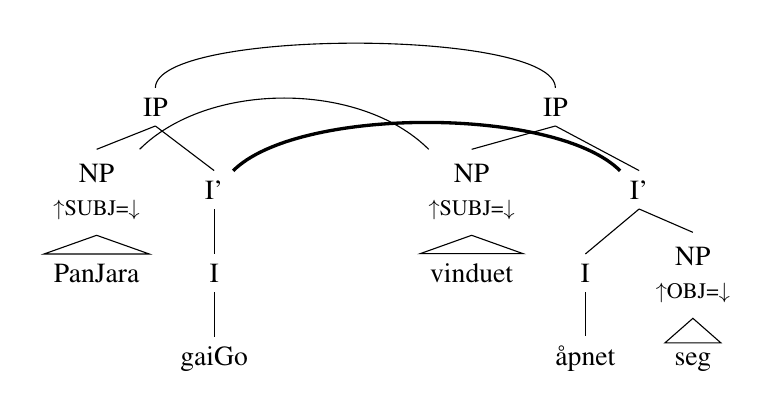
\begin{tikzpicture}
\Tree [.\node(IPs){IP}; 
  [.\node(NPs){\proj{NP}{\ua SUBJ=\da}}; \edge[roof]; {PanJara} ] 
  [.\node(I's){I'};  [.\node(Is){I};    \node(gaiGo){gaiGo};  ]
  ] ]
     \begin{scope}[shift={(2in,0in)}]
\Tree [.\node(IPt){IP}; 
  [.\node(NPt){\proj{NP}{\ua SUBJ=\da}}; \edge[roof]; {vinduet} ] 
  [.\node(I't){I'};  [. \node(It){I}; \node(åpnet){åpnet};  ]
       [.\proj{NP}{\ua OBJ=\da} \edge[roof]; {seg} ] ] ]
\end{scope}
 \draw[-] (IPs)..controls +(north:1) and +(north:1) .. (IPt) ;
  \draw[-,very thick] (I's)..controls +(north east:1.5) and +(north west:1.5) .. (I't) ;
%  \draw[dashed,-] (Is)..controls +(north east:1) and +(north west:1) .. node[midway,sloped]{$\times$}(It) ;
 \draw[-] (NPs)..controls +(north east:2) and +(north west:2) .. (NPt) ;

\end{tikzpicture}
\caption{Delvis mogleg lenkjing av underordna c-strukturnodar mellom georgisk og bokmål}
 \label{fig:PanJara-gaiGo}
\end{figure}


\citet[s.~77]{dyvik2009lmp} definerer i denne samanhengen
omgrepet \emph{lenkja leksikalske nodar}, $LL$, kor $LL(n)$ er mengda av
nodar dominert av $n$ som har ei ordlenkje. For å lenkje
c-strukturnodane $n_s$ og $n_t$, som er i lenkja funksjonelle domene,
må alle nodane i mengda $LL(n_s)$ vere lenkja til nodar i
$LL(n_t)$. Ulenkja nodar under $n_s$ og $n_t$ står ikkje i vegen for
lenkjing av $n_s$ og $n_t$, men dei to mengdene kan ikkje vere tomme.

Dette kravet gjer at ein ikkje treng krav \ref{krav:c-tentativt}, og
vil gi ei mange-mange-lenkje mellom alle nodane i dei to funksjonelle
domena til \emph{gaiGo-åpnet} i figur \ref{fig:gaiGo}. Viss me skriv ei
f-strukturlenkje som eit ordna par mellom PRED-verdien på kjeldesida
(georgisk, med subskript $_s$) og PRED-verdien på målsida (norsk, med
subskript $_t$) får me
$LL(IP_s)=LL(I'_s)=LL(I_s)=\{(\textbf{ga-Geba},\textbf{åpne})\}=LL(IP_t)=LL(I'_t)=LL(I_t)$
kor \emph{det} og \emph{seg} er ulenkja på både c-strukturnivå og ordnivå\footnote{\label{fn:LL-ordlenkje} Merk at orda \emph{det} og \emph{seg} måtte definerast som ulenkja for
        at denne definisjonen skulle fungere, noko som krev at ein nyanserer
        krav \ref{krav:f-links-words} litt. Viss me hadde definert
        \emph{det} og \emph{seg} som mange-ein-lenkja (med \emph{åpnet}) inn i
        \emph{gaiGo}, ville me fått same resultat som det krav
        \ref{krav:c-pro} i del \ref{SEC:c-strengare} gir.
        Viss georgisk er kjeldespråket
        ($n_s$, norsk: $n_t$) blir
        $LL(IP_s)=LL(I'_s)=LL(I_s)=\{(\text{gaiGo},\text{det}),(\text{gaiGo},\text{åpnet}),(\text{gaiGo},\text{seg})\}=LL(IP_t)$.
        Mengdene
        $LL(I'_t)=\{(\text{gaiGo},\text{åpnet}),(\text{gaiGo},\text{det})\}$
        og $LL(I_t)=\{(\text{gaiGo},\text{åpnet})\}$ på den norske
        sida har då ikkje korresponderande mengder på georgisk og blir
        ikkje lenkja. }.

\fxnote{TODO: diskutere litt meir forskjellane på desse alternativa}

\subsection{Eit strengare lenkjingskriterium}
\label{sec-3.7.2}

\label{SEC:c-strengare}

Sidan det er mogleg å ønskje seg å ikkje lenkje I'- og I-nodane i
\ref{fig:gaiGo}, gir eg her ein måte å formalisere dette på.

For å tillate lenkjene i figur \ref{fig:enkel-c-lenkje}, men ikkje dei
stipla lenkjene i figur \ref{fig:gaiGo}, ville det vore nok å krevje
at søsternodane var lenkja. I figur \ref{fig:enkel-c-lenkje} kan
I-nodane lenkjast fordi objekta er lenkja, I'-nodane fordi subjekta er
lenkja. I figur \ref{fig:gaiGo} kan dei norske I'- og I-nodane ikkje
lenkjast med noko fordi søstrene deira ikkje er lenkja.
Men dette blir for strengt. Det kan t.d. vere gode uavhengige grunnar
til å ha ein mellomliggande S-node før objektet på norsk, kor S er i
same funksjonelle domene som IP, medan det kanskje finst uavhengige grunnar
for å \emph{ikkje} gjere dette på andre språk. Figur
\ref{fig:enkel-c-lenkje-med-S} demonstrerer denne situasjonen. Her kan
ikkje S lenkjast til objektet sidan dei ikkje er i same funksjonelle
domene, men me vil jo likevel lenkje I-nodane; så eit krav om lenkja
søsternodar blir for strengt.

\begin{figure}[htp]
\centering
  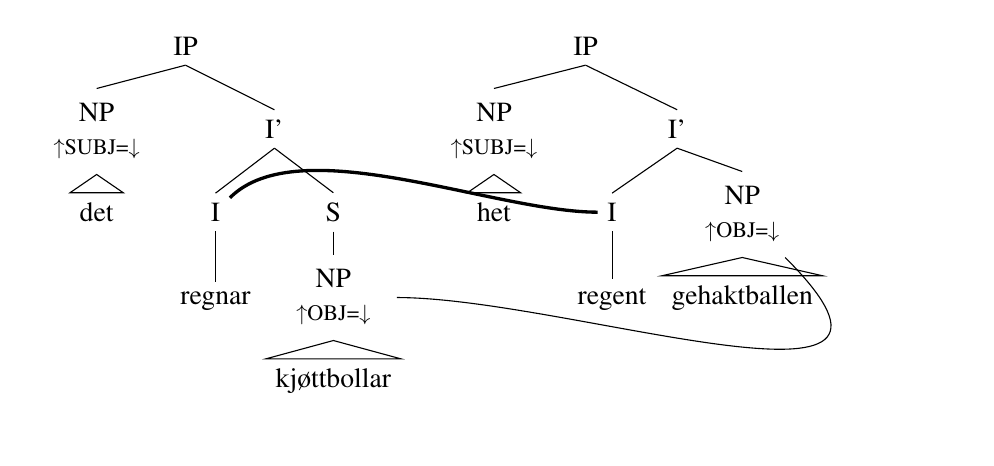
\begin{tikzpicture}
  \Tree  [.\node(IPs){IP};  [.\node(SUBJs){\proj{NP}{\ua SUBJ=\da}}; \edge[roof]; {det} ]
                            [.\node(I's){I'};
                                    [.\node(Is){I}; {regnar} ]
                                    [.S [.\node(OBJs){\proj{NP}{\ua OBJ=\da}}; \edge[roof]; {kjøttbollar} ] ] ] ]
      \begin{scope}[shift={(2in,0in)}]
  \Tree  [.\node(IPt){IP};  [.\node(SUBJt){\proj{NP}{\ua SUBJ=\da}}; \edge[roof]; {het} ] 
                            [.\node(I't){I'}; 
                                    [.\node(It){I}; {regent} ]
                                    [.\node(OBJt){\proj{NP}{\ua OBJ=\da}}; \edge[roof]; {gehaktballen} ] ]   ]
\end{scope}
  \draw[-,very thick] (Is)..controls +(north east:1.5) and +(west:1.5) .. (It) ;
  \draw[-] (OBJs)..controls +(east:3) and +(south east:4) .. (OBJt) ;
\end{tikzpicture}
   \caption{I-nodane bør lenkjast sjølv om søsternodane ikkje er
   lenkja (norsk og nederlandsk)}
   \label{fig:enkel-c-lenkje-med-S}
  \end{figure}

Me treng altså eit litt meir nyansert krav. Som nemnt i fotnote
\ref{fn:LL-ordlenkje} går det an å få til dette ved ein kombinasjon av
konseptet om lenkja leksikalske nodar og å krevje at orda \emph{det},
 \emph{åpnet} og \emph{seg} i figur \ref{fig:gaiGo} er mange-mange-lenkja på
ordnivå til \emph{gaiGo}, sidan dei er lenkja til subjekt, predikat og
objekt av \emph{gaiGo} på f-strukturnivå. 

Men viss me vil unngå å referere til ordlenkjer, går det au an å
definere kravet i form av f-strukturlenkjer på preterminale
nodar\footnote{Då kan me au representere mange-til-mange-ordlenkjer som
        «udelelege», $(\{\text{gaiGo}\},\{\text{det,åpnet,seg}\})$
        blir den einaste ordlenkja i dømet over, sidan me ikkje må
        samanlikne ordlenkjene frå $IP_t$, $I'_t$ og $I_t$. }:

\ex. \label{krav:c-pro} For å lenkje c-strukturnodane $n_s$ og
     $n_t$:\\
     La $l_c(f)$ vere mengda som inneheld
     f-strukturlenkja til $f$, \emph{og} f-strukturlenkjene til alle
     argument $a$ av $f$ som ikkje har c-strukturnodar, dvs. kor
     $\phi^{-1}(a)=\emptyset$.
     La $L_c(n)$ vere mengda av $l_c(\phi(n'))$ for alle
     f-strukturlenkja preterminale $n'$ som er dominert av $n$.
     $n_s$ og $n_t$ kan lenkjast om $L_c(n_s)=L_c(n_t)$.

I figur \ref{fig:PanJara-gaiGo} har me då følgjande situasjon:\\
\\$L_c(IP_s)=\{(\textbf{PanJara},\textbf{vindu}),(\textbf{ga-Geba},\textbf{åpne}),(\textbf{pro},\textbf{seg})\}=L_c(IP_t)$
\\$L_c(I'_s)=\{(\textbf{ga-Geba},\textbf{åpne}),(\textbf{pro},\textbf{seg})\}=L_c(I'_t)$
\\$L_c(I_s)=\{(\textbf{ga-Geba},\textbf{åpne}),(\textbf{pro},\textbf{seg})\}
\neq \{(\textbf{ga-Geba},\textbf{åpne})\}=L_c(I_t)$\\

Dette vil seie at krav \ref{krav:c-pro} gir lenkjer mellom
IP-nodane og I'-nodane, men ikkje mellom I-nodane. I figur
\ref{fig:gaiGo} vil ikkje ein gong I'-nodane få ei lenkje, sidan den
norske I'-node dominerer 
$\{(\textbf{ga-Geba},\textbf{åpne}),(\textbf{pro},\textbf{seg})\}$
medan den georgiske I'-node dominerer
$\{(\textbf{pro},\textbf{det}),(\textbf{ga-Geba},\textbf{åpne}),(\textbf{pro},\textbf{seg})\}$,
det same som IP-nodane.

Merk at om me omdefinerer $l_c(f)$ til å ikkje innehalde
f-strukturlenkjer til argument av $a$, vil krav \ref{krav:c-pro} gi
same c-strukturlenkjer som kravet frå \cite{dyvik2009lmp}, men
definert i form av f-strukturlenkjer på preterminale nodar.
\subsection{Funksjonelle c-strukturnodar}
\label{sec-3.7.3}

\label{SEC:fnord}

Ikkje alle ord tilsvarer PRED-element i f-strukturen, dette gjeld
typisk funksjonsord (t.d. \emph{som}, \emph{at}). \fxnote[inline,nomargin]{...og
desse vil me lenkje kvifor? i kva situasjonar? TODO diskuter.}
Ved endosentrisitetsprinsippa
til \citet{bresnan2001lfs} er komplementet til funksjonelle kategoriar
(C, I, P) ein funksjonell ko-kjerne, det er altså komplementet som gir
PRED-elementet i dette funksjonelle domenet.

Problemet med å nytte krava nemnt over i dette tilfellet er at nodar
over funksjonsord er i det same funksjonelle domenet som komplementet,
og nodane over funksjonsorda tilføyer ikkje ei ny PRED-lenkje som kan
dele opp treet slik me gjorde tidlegare. Så me må utvide prinsippa for
å dele opp c-strukturtreet i buntar som dominerer same mengd med
lenkjer.

Ord som ikkje projiserer PRED-lenkjer kan likevel ha
LPT-korrespondanse og bestå krava på ordnivå, men når me skal lenkje
desse på c-strukturnivå må me sjekke ordkrava direkte (me kan ikkje gå
via nokon f-strukturlenkjing). LPT-kravet gir oss eit utgangspunkt for
lenkjing.

Viss begge språk har funksjonsord, men funksjonsord som ikkje kan
sjåast på som moglege omsetjingar (t.d. \emph{fordi} og \emph{whether}), bør me
nok ikkje ein gong lenkje komplementa, sidan funksjonsorda då gjer at
komplementa speler ulike roller i omgivnadene\footnote{Skal ein lenkje ordet \emph{som} (utan PRED) med ordet \emph{which} (med
        PRED)? Viss krava elles er oppfylt, kan det kanskje vere
        informativt med ein type «defekt» lenkje, sjølv om berre det
        eine ordet blir rekna for å vere eit innhaldsord. Frasane til
        deira funksjonelle domene vil uansett kunne lenkjast viss dei andre
        krava er oppfylte. }. Samtidig vil me
ikkje at eit manglande funksjonsord på det eine språket skal hindre
lenkjing av komplementa, sidan det kan hende at funksjonsordet ikkje
er krevd på det språket (eventuelt kjem dette fram som korrespondansar
i f-strukturtrekk, eg har ikkje teke høgd for korrespondansar mellom
andre f-strukturelement enn PRED i denne oppgåva).

Me kan krevje at komplementa er lenkja for å sikre at me ikkje lenkjer
nodar som står i ulike konstekstar (me vil ikkje lenkje \emph{at} i «han
såg at det gjekk bra» med \emph{that} i «he saw that she drew a picture»),
jamfør kravet om lenkja argument for lenkja predikat i del
\ref{SEC:lik-argstr}.

Desse ønskene kan me formalisere slik:

\ex. \label{fnordkrav} Krav for lenkjing av funksjonelle kategoriar i c-strukturen:
\a. Gitt ei mogleg lenkjing av FP og GP, kor F og G er funksjonelle
    kategoriar der komplementa elles kan lenkjast,
    tolk LPT-korrespondansen mellom orda under F' og G' som eit
    medlem av lenkjemengda $L_c$ (evt. $LL$), kor denne må vere lik
    for at FP og GP skal kunne lenkjast, då kan me au lenkje F' og G'.
\b. Gitt ei mogleg lenkjing av FP og XP, der F er ein funksjonell
    kategori, medan X er ein ikkje-funksjonell kategori, ignorerer me
    den funksjonelle kategorien i c-strukturlenkjinga. Sidan det ikkje
    er nokon forskjell i $L_c$ (evt. $LL$) mellom FP og F', er F' medlem
    av nodemengden som blir lenkja til XP.

Om \Last[a] er oppfylt, kan me få samanstillinga vist i figur
\ref{fig:fnord}. Her vil dei funksjonelle domena til CP og CP
kvar kunne delast opp i to deler, kor den funksjonelle delen har
LPT-korrespondanse medan komplementa er lenkja på
f-strukturnivå. Lenkjemengdene under CP-nodane er like, og dei under
C-nodane er like.

(Alle nodane under S vist i dei to trea er i same funksjonelle domene,
så om dei funksjonelle domena er lenkja, vil krav
\ref{krav:subnode-f-lenkja} vere oppfylt kva gjeld CP-komplementa --
lenkjinga går ikkje ut over dei funksjonelle domena, medan
krav \ref{krav:c-pro} er dekkja for S-nodane med unntaket over.)

  \begin{figure}[htp]
   \centering
  
  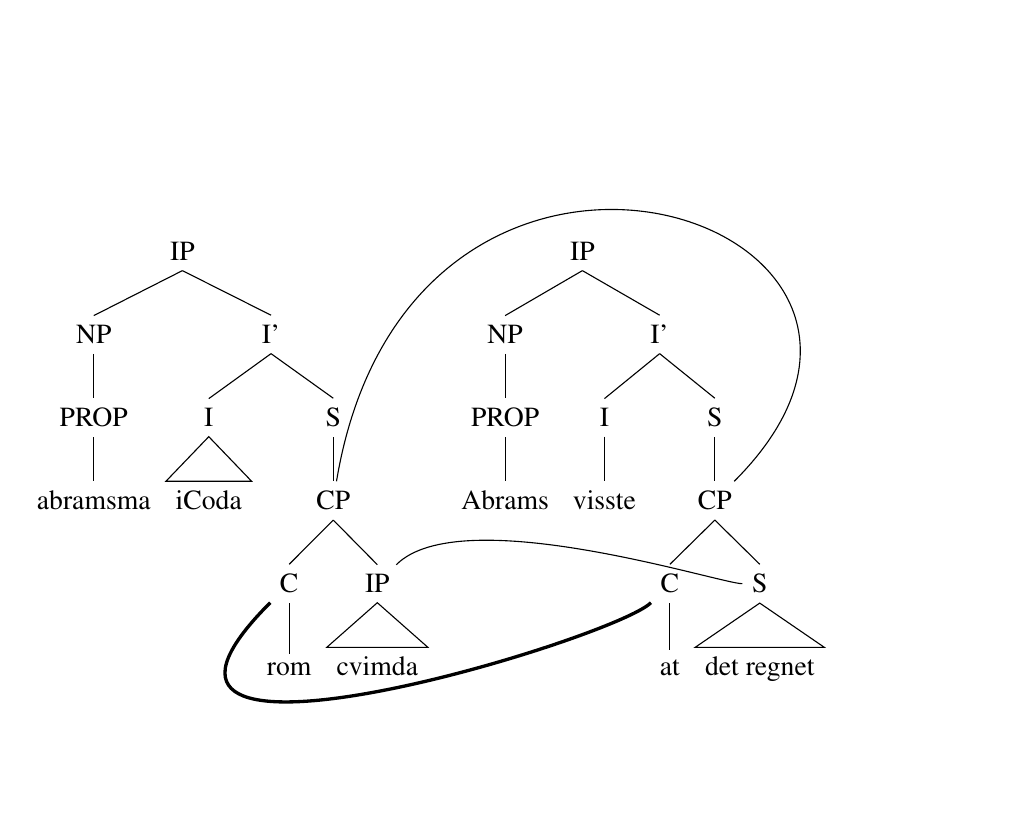
\begin{tikzpicture}
  \Tree
  [.IP
    [.NP [.PROP abramsma ] ] 
    [.I' [.I \edge[roof]; {iCoda} ]
             [.S [.\node(CPs){CP};
                  [.\node(Cs){C};  rom ]
                  [.\node(IPs){IP}; \edge[roof]; {cvimda} ]]]]]
      \begin{scope}[shift={(2in,0in)}]
  \Tree
  [.IP
    [.NP [.PROP Abrams ] ]
     [.I' [.I visste ]
              [.S  [.\node(CPt){CP};
                   [.\node(Ct){C};  at ] 
                   [.\node(St){S}; \edge[roof]; {det regnet} ]]]] ]
  \end{scope}                      
  \draw[-] (CPs)..controls +(1,6) and +(north east:5) .. (CPt) ;
  \draw[-] (IPs)..controls +(north east:1.5) and +(west:0.5) .. (St) ;
  \draw[-,very thick] (Cs)..controls +(south west:4) and +(south west:1) .. (Ct) ;
  \end{tikzpicture}
  \caption{Mogleg samanstilling av funksjonelle c-strukturnodar mellom georgisk og norsk (bokmål)}
   \label{fig:fnord}
  \end{figure}

Der det eine språket har eit funksjonsord og det andre språket ikkje
krever det, bryr me oss ikkje om funksjonsordet. For å sjekke noko
slikt må me som nemnt sjå på andre trekk enn PRED i f-strukturane,
noko som blir utanfor denne oppgåva; men om me hadde sjekka slike
f-strukturkorrespondansar kunne me unngått kravet om
LPT-korrespondanse og i staden nytta informasjon frå f-strukturane til
lenkjing av funksjonelle kategoriar. Utan å ha slike mekanismar på
plass blir f-strukturlenkjinga avhengig av c-strukturforhold, og i
implementasjonen min har eg difor lagt mindre vekt lenkjing av
funksjonelle kategoriar.

\section{\textbf{SKRIV} Rangering}
\label{sec-3.8}

   \label{SEC:rangering}
(meir om dette i del \ref{SEC:impl-f-rangering})

\section{\textbf{SKRIV} Oppsummering av krava}
\label{sec-3.9}

\chapter{Implementasjonen av \texttt{lfgalign}}
\label{sec-4}

\label{SEC:implementasjon}

For å finne ut av kor godt krava i forrige kapittel fungerer til å
avgrense kva for lenkjer som er moglege, har eg implementert dei etter
beste evne i eit Lisp\footnote{Dette språkvalet kan gjere eventuell integrering med andre
        LFG-system lettare (Common Lisp er m.a. nytta i LFG
        Parsebanker \citep{rosen2009lpt}). }-program.

\fxnote{intro TODO, kanskje noko om kva eg faktisk har fått ut av
implementasjonen} Ei implementering gjer det svært synleg om det finst
manglar i eit formelt krav, eller om noko ikkje er godt nok
spesifisert.

Programmet \texttt{lfgalign}\footnote{Tilgjengeleg frå \href{http://github.com/unhammer/lfgalign}{http://github.com/unhammer/lfgalign} som fri og
       open programvare under GNU General Public License. } tek inn LFG-analysane av to
setningar som me av uavhengige grunnar trur er omsetjingar av
kvarandre. LFG-analysane må vere disambiguerte og i Prolog-formatet
frå XLE\footnote{Formatet er dokumentert på
       \href{http://www2.parc.com/isl/groups/nltt/xle/doc/xle.html}{http://www2.parc.com/isl/groups/nltt/xle/doc/xle.html}. Importeringa
       til Lisp-strukturar handterer «pakka representasjonar» og
       kjenner igjen ekvivalensforhold (t.d. der fleire
       $\phi$-variablar refererer til same f-struktur, eller fleire
       Prolog-variabler refererer til same analyseval); men filene eg
       har testa utnyttar ikkje det fulle spennet til formatet, så det
       finst ganske sikkert feil. }. Programmet les inn dei to filene og opprettar ein
intern representasjon av LFG-analysen.  \fxnote{treng eg ein eigen del
om LPT i dette kapittelet? Implementasjonen er jo veldig enkel
iallfall.}

Me kan i tillegg gi programmet informasjon om kva for ord-omsetjingar
me ser på som lingvistisk prediktable. Intensjonen er at dette kan
vere informert av omsetjingstabellen frå eit automatisk
ordsamanstillingsprogram, eller av handskrivne omsetjingsordbøker.

Programmet byrjar lenkjinga med f-strukturane. Ei
f-struktur\emph{samanstilling} er ei mengd med \emph{lenkjer} mellom
individuelle f-strukturar. Resultatet av lenkjinga på dette nivået kan
vere tvitydig: sidan det ofte finst fleire måtar å lenkje argument og
adjunkt på, får me i første omgang mange samanstillingar mellom
kjelde- og mål-f-strukturar.

Difor rangerer me f-struktursamanstillingane, og den beste sender me
vidare til c-struktursamanstillinga. Denne delen av programmet gir ut
éi, utvitydig mengd med mange-til-mange-lenkjer mellom c-strukturane
(her treng me ingen rangering). Nodane i kvar av desse
mange-til-mange-lenkjene definerer no den endelege
frasesamanstillinga.

Nedanfor går eg gjennom detaljane rundt dei relevante delene av
programmet.

\section{Lenkjer mellom f-strukturar}
\label{sec-4.1}

\label{SEC:impl-f-lenkjing}

Hovudalgoritmen for lenkjing mellom f-strukturar er vist i kodefigur
\ref{algo:f-align}. Funksjonen \texttt{f-align} returnerer ei mengd med
moglege samanstillingar. Kvar samanstilling er ei mengd med par av
f-strukturar\footnote{Eigentleg eit slag avgjerdstre; kvart element er eit par, kor
        første element er lenkja mellom dei yttarste f-strukturane, og
        andre element er dei moglege samanstillingane for dei indre
        strukturane. Denne strukturen kan vere nyttig for å rangere
        samanstillingar, og \texttt{f-align} blir mykje meir oversiktleg av å
        jobbe med eit slikt tre. Ein funksjon \texttt{flatten} omformar det
        ferdige treet til ei enkel liste med samanstillingar, kor kvar
        samanstilling er ei flat liste med lenkjer mellom
        f-strukturar. }. Eit par $(F_s,F_t)$ representerer ei lenkje frå
ein f-struktur på kjeldespråket, til ein f-struktur på målspråket. Me
går ut frå at dette paret har LPT-korrespondanse\footnote{Når eg her skriv at to f-strukturar har LPT-korrespondanse,
        meiner eg sjølvsagt at ordformene til PRED-verdien til kvar
        f-struktur har LPT-korrespondanse. }, dette blir
sjekka før alle kall på \texttt{f-align}. Der me ikkje har informasjon om
LPT-korrespondanse mellom to ord (orda er ukjende), er lenkjing
lov. Pro-element og substantiv kan alltid lenkjast med kvarandre.
\fxnote{TOGROK: kan me i tillegg sjekke om funksjonelle nodar i same
f-domene som PRED-ordformen har LPT-korrespondanse?}

Hjelpefunksjonen \texttt{argalign} (som igjen kallar \texttt{argalign-p}, vist i
kodefigur \ref{algo:argalign-p}) gir alle moglege
«argumentpermutasjonar», dvs. moglege kombinasjonar av lenkjer mellom
argumenta til $F_s$ og $F_t$ som tilfredsstiller kravet om
LPT-korrespondanse, men utan å sjekke at desse argumenta igjen kan
samanstillast. Funksjonen prøver å lenkje kvart argument til eit
argument eller eit adjunkt, men gir ingen lenkjer mellom to adjunkt
(sjå del \ref{SEC:impl-adjalign} nedanfor om dette). Funksjonen gir
heller ikkje kombinasjonar der minst eitt argument ikkje er lenkja --
alle kombinasjonane må inkludere alle argument frå $F_s$ og $F_t$,
jf. krav (iii) og (iv) i \citet[s.~75]{dyvik2009lmp}. Elles er krav
(i) er tautologisk oppfylt, medan me som nemnt føreset at krav (ii) er
oppfylt før alle kall på \texttt{f-align}.

Eit døme: viss $F_s$ har argumenta \SUBJs og \OBJs og ingen adjunkt,
og $F_t$ har argumentet \SUBJs og eitt adjunkt \ADJ, der alle
ord-omsetjingar er moglege, vil \texttt{argalign} gi dei to samanstillingane
$\{(\SUBJ,\SUBJ), (\OBJ,\ADJ)\}$ og $\{(\SUBJ,\ADJ),
(\OBJ,\SUBJ)\}$. Viss adjunktet til $F_t$ ikkje fantest, eller ikkje
hadde LPT-korrespondanse med nokon av argumenta til $F_s$, ville me
ikkje fått nokon samanstillingar; medan viss paret $(\SUBJ,\SUBJ)$
ikkje hadde LPT-korrespondanse og alt anna var likt, ville me berre
fått den siste samanstillinga.

Funksjonen \texttt{f-align} går så gjennom kvar lenkje i kvar
argumentpermutasjon, og prøver å kalle \texttt{f-align} på alle
lenkjene. Sidan lenkjene som \texttt{argalign} gir har LPT-korrespondanse,
vil alle f-strukturane i dei rekursive kalla i \texttt{f-align} ha
LPT-korrespondanse. Eit rekursivt kall kan gi nye samanstillingar i
dei indre f-strukturane, viss dei relevante krava er oppfylte.

Det er mogleg at ei lenkje frå éi samanstilling kan finnast i andre
samanstillingar, me unngår dobbeltarbeid ved å lagre alle delvise
samanstillingar i tabellen $aligntable$. Dette føreset at
\texttt{f-align}$(s,t)$ er uavhengig av konteksten rundt; t.d. må
mengda av samanstillingar som kjem ved å lenkje subjektet til $F_s$
mot subjektet til $F_t$ vere uavhengig av om objektet til $F_s$ er
lenkja mot eit objekt eller eit adjunkt osb. av $F_t$. \fxnote{TODO:
nemne føresetnaden om uavhengnad i kapittel 3}

      \SetKwComment{Comment}{ // }{}
     \SetKwInOut{Input}{usage}
  
     \begin{algorithm}[]
      \caption{f-align($F_s$, $F_t$)}
      \label{algo:f-align}
      
      $alignments \gets \emptyset$  \;
      \ForAll{argperm in argalign($F_s$, $F_t$)} {
        $p \gets \emptyset$ \;
         \ForAll{$A_s$, $A_t$ in argperm} {
           \uIf{not(aligntable[$A_s$,$A_t$])} {
           aligntable[$A_s$,$A_t$] $\gets$ f-align($A_s$, $A_t$)\;
           }
          \uIf{aligntable[$A_s$,$A_t$]}{add aligntable[$A_s$,$A_t$] to $p$\;}
          \uElse{add $(A_s, A_t)$ to $p$}
        }
        add $p$ to $alignments$ \;
        \ForAll{adjperm in adjalign(argperm, $F_s$, $F_t$)} {
          $a \gets$ copy-of($p$) \Comment*[r]{optional adjunct links}
          \ForAll{$A_s$, $A_t$ in adjperm}{
            \uIf{not(aligntable[$A_s$,$A_t$])} {
              aligntable[$A_s$,$A_t$] $\gets$ f-align($A_s$, $A_t$)\;
            }
            \uIf{aligntable[$A_s$,$A_t$]}{add aligntable[$A_s$,$A_t$] to $a$\;}
            \uElse{add $(A_s, A_t)$ to $a$}
          }
          add $a$ to $alignments$ \;
        } % adjperm in adjalign
       } % argperm in argalign
       \Comment{loop through adjalign if no arguments exist}
       \lIf {$alignments=\emptyset$}{ \Return $\emptyset$ \Comment*[l]{Fail} }
       \lElse{ \Return $((F_s, F_t), alignments)$ \; }
       \end{algorithm}    
    
    
      \begin{algorithm}[]
      \caption{argalign-p($args_s$, $adjs_s$, $args_t$, $adjs_t$)}
      \label{algo:argalign-p}
    
      \Input{Kalt av argalign slik: \\ argalign-p(arguments($F_s$),
      adjuncts($F_s$), arguments($F_t$), adjuncts($F_t$))}
      \BlankLine
      
     $a \gets \emptyset$\;
     \uIf{$args_s$} {
           $s \in args_s$\;
           \ForAll{$t \in args_t$ \textbf{where} LPT($s$,$t$)} {
               \lForAll{$p \in$ argalign-p($args_s-\{s\}$, $adjs_s$, $args_t-\{t\}$,$adjs_t$)}{
  add $\{(s,t)\} \bigcup p$ to $a$\;
             }
            }
           \ForAll{$t \in adjs_t$ \textbf{where} LPT($s$,$t$)} {
               \lForAll{$p \in$ argalign-p($args_s-\{s\}$, $adjs_s$, $args_t$,$adjs_t-\{t\}$)}{
  add $\{(s,t)\} \bigcup p$ to $a$\;
                }
           }
             \Return $a$\;
         }
          \uElseIf{$args_t$} {
            \uIf{$adjs_s$}{
                $s \in adjs_s$\;
           \ForAll{$t \in args_t$ \textbf{where} LPT($s$,$t$)} {
               \lForAll{$p \in$ argalign-p($args_s$, $adjs_s-\{s\}$, $args_t-\{t\}$,$adjs_t$)}{
  add $\{(s,t)\} \bigcup p$ to $a$\;
             }
            }
             \Return $a$\;
        }\uElse{
              \Return $\emptyset$  \Comment*[l]{Fail}
            }
          }
        \uElse {
          \Return \{$\emptyset$\} \Comment*[l]{End}
        }     
      \end{algorithm}

Sjølv om det er krav om LPT-korrespondanse mellom kvart argument og
eit argument/adjunkt for å lenkje $F_s$ og $F_t$, er det ikkje noko
krav om at alle para i ein argumentpermutasjon tilfredsstiller alle
lenkjingskrava. Viss \texttt{f-align}$(\OBJ,\ADJ)$ frå dømet over gir
null, og ikkje kan lenkjast (t.d. fordi \ADJs hadde eitt argument, og
\OBJs ingen argument/adjunkt), medan \texttt{f-align}$(\SUBJ,\SUBJ)$
kan lenkjast, vil \texttt{f-align} likevel returnere samanstillinga som
inneheld $(\OBJ,\ADJ)$ og $(\SUBJ,\SUBJ)$. Me kan sjå i $aligntable$
for å finne ut av om kvar av f-strukturane kunne lenkjast; i dette
tilfellet vil $aligntable[\OBJ,\ADJ]$ vere tom.

\fxnote{TODO: forskjellen mellom LPT-krav og rekursjonskrav på argument må
inn i kapittel 3}

Om me i tillegg krev at substrukturar kan samanstillast kan me
utelukke lenkjing av f-strukturane $F_s$ og $F_t$ i \Next under:

{\avmoptions{}

\ex. \a.  \begin{avm}  \sort{$F_s$}{\[ {\sc pred} `{\bf planlegge}<{\it eg},[1:{\it gi}]>'\\
  {\sc xcomp} \sort{$^{1}$}{\[ {\sc pred} `{\it gi (opp)}'\]} \]}  \end{avm}
  \b.\begin{avm} \sort{$F_t$}{\[ {\sc pred} `{\bf plan}<{\it I},[2:{\it give}]>'\\
  {\sc xcomp} \sort{$^{2}$}{\[ {\sc pred} {\bf give}<{\it I},{\it him},{\it it}>' \]} \]} \end{avm}

}

Men det kan vere at me ikkje \emph{vil} krevje dette i alle moglege
tilfelle. Ei tryggare løysing er å rangere ulike løysingar i
etterkant, ved å spørje etter dei argumentsamanstillingane som har
flest medlem i $aligntable$, dette kjem eg tilbake til i
\ref{SEC:impl-f-rangering} nedanfor.
\subsection{Overflødige adverbial}
\label{sec-4.1.1}

   \label{SEC:impl-adjalign}

Argumentpermutasjonane frå \texttt{argalign} prøver som nemnt ikkje reine
adjunkt-adjunkt-lenkjer, sidan me ikkje vil forkaste lenkjing av $F_s$
og $F_t$ berre på grunn av at ikkje alle adjunkt kunne lenkjast. Men
når me har prøvd ein argumentpermutasjon, kan me lage ein kopi av
denne som i tillegg inneheld lenkjer mellom «overflødige» adverbial,
altså dei adjunkt-adjunkt-lenkjene som \texttt{argalign} ikkje
prøver. Hjelpefunksjonen \texttt{adjalign} (ikkje vist her
\fxnote[inline,nomargin]{TODO: implementere :->}) konstruerer moglege
permutasjonar av lenkjer mellom adjunkt som ikkje er inkludert i
$argperm$, og \texttt{f-align} prøver desse rekursivt på same måte som med
argumentlenkjene. \fxnote{og så er det spørsmålet om me kan lenkje
adjunkt på ulike nivå i f-strukturane} Lenkjene blir lagt til ein
\emph{kopi} av argumentpermutasjonane, sidan det ikkje er sikkert at me
ønskjer å lenkje alle adjunktdøtre. Viss me har to overflødige adjunkt
på kvar side, og kravet om LPT-korrespondanse er dekkja for alle fire
moglege par, får me seks moglege permutasjonar, sidan me inkluderer
dei fire permutasjonane der eitt adjunktpar er ulenkja.

Viss $F_s$ og $F_t$ ikkje hadde argument i det heile teke, går me au
gjennom moglege permutasjonar av adjunktdøtre, på same måte (ikkje
vist i kodefigur \ref{algo:f-align}).

\subsection{\textbf{SKRIV} Funksjonsord utan LPT-korrespondanse bør eigentleg hindre f-strukturlenkjing}
\label{sec-4.1.2}

\subsection{\textbf{SKRIV} Når f-lenkjene ikkje er 1-1}
\label{sec-4.1.3}

\fxnote{Dette må 1. spesifiserast (kap.3), og 2. implementerast...}
\subsubsection{kausativ}
\label{sec-4.1.3.1}

\subsubsection{preposisjonsobjekt}
\label{sec-4.1.3.2}

``sigaretten'' og ``sigaretze'' er ikkje på same nivå i dei respektive
f-strukturane nedanfor:
\begin{verbatim}
 0[ PRED vedde<28,29,27,30>
    29[ PRED sigarett<> ] ]
\end{verbatim}


\begin{verbatim}
 0[ PRED da-najleveba<37,10,46>
    ADJUNCT { 2 }
    2[ ze<5>
       OBJ 5[ sigareti ] ] ]
\end{verbatim}


Men dette er fordi sigaretze er \underline{adjunkt}, og i følgje fotnote 3 i
\citet{dyvik2009lmp} er P(ADJ) lik den semantiske formen til
\underline{preposisjonsobjektet} til ADJ. (Er dette heilt enkelt? Kan me ha
adjunkt med fleire «preposisjonsargument»?)

I motsetning til å endre på P(ADJ) slik at pred-verdien til eit
adjunkt hoppar over preposisjonar og inn i preposisjonsobjekt, har eg
i implementasjonen min gjort det slik at funksjonen som henter ut \emph{f-strukturen} til adjunkt-døtre av ein f-struktur hoppar over
preposisjonsobjekt (m.a. fordi ved eit kall P(X) kan ikkje P vite om X
er eit adjunkt eller argument).

Sjå au del \ref{SEC:merge-daughters}.

\subsection{Kan me gjere f-struktursamanstillinga bottom-up?}
\label{sec-4.1.4}

  %     \begin{quotation}
  %    Any sufficiently complex problem needs to be coded three times.\\
  % \begin{minipage}{0.8\textwidth}
  % \begin{flushright}
  %        (ukjend, via Steve Gibson)
  % \end{flushright}
  % \end{minipage}
  %    \end{quotation}
Ein alternativ metode for lenkjing av f-strukturane er å byrje med
alle logisk moglege permutasjonar av LPT-korrespondansar, og så sile
ut dei som ikkje svarer til krava. Prosessen ville nok blitt mykje
meir oversiktleg på denne måten, sidan det då berre er snakk om å
sjekke krav for kvar enkelt lenkje.  Men ein slik metode er vanskeleg
i praksis; når avskjeringa skjer så seint, blir det alt for mange
moglege kombinasjonar for lengre setningar med mange ukjende ord til
at ein vanleg datamaskin kan halde styr på dei.

Me må i alle tilfelle vere klar for ei setning der alle ord er ukjende
(me har ingen informasjon om LPT-korrespondanse), slik at kvart
kjeldeord kan lenkjast til kvart målord. Viss begge setningane er 4 ord,
får me 16 moglege samanstillingar der alle ord er med i nøyaktig éi
lenkje ($2^l$, kor $l$ er setningslengd). Men ofte har me
null-lenkjer, me må altså i tillegg tillate samanstillingar der minst
eitt ord er ulenkja, utan at me treng å vite kva for ord det er; med
desse kortare listene inkludert får me endå fleire moglege
samanstillingar per setning (4 ord gir 26, 8 ord gir 2186 moglege
samanstillingar). Sjølv om me heile tida vel dei samanstillingane som
lenkjar flest ord, ville maskinen raskt fått problem. I tillegg har me
problemet med 1-mange-lenkjer, som skaper endå fleire moglege
samanstillingar.

Ein sideverknad av å byrje med ytre lenkjer og gå innover (prosessen
skildra i del \ref{SEC:impl-f-lenkjing}) er at me automatisk unngår å
prøve «kryssande» lenkjer, t.d. å lenkje $F_s$ med \XCOMPs av $F_t$, og
\XCOMPs av $F_s$ med $F_t$ (denne kombinasjonen av lenkjer vil jo vere
ein del av alle logisk moglege permutasjonar). Me får au prioritert å
lenkje ytre element, som jo er sikrare lenkjer: gitt to f-strukturar
for setningar der alt me veit om lenkjinga er at \emph{setningane} er
omsetjingar av kvarandre, vil dei to ytre f-strukturane ha størst
sjanse for å korrespondere med kvarandre. For kvart steg du går
innover må du multiplisere inn sjansen for å trå feil i
argumentpermutasjonane.

\section{\textbf{SKRIV} Rangering}
\label{sec-4.2}

\label{SEC:impl-f-rangering}

\fxnote[inline,nomargin]{Rangering er ikkje implementert enno (akkurat no gir
rank(f-alignments) berre ut første samanstilling.)}
Rangering foregår etter ulike kriterium. Her er eit par forslag:
\subsection{rekursivt lenkja > ulenkja, men LPT}
\label{sec-4.2.1}

    $aligntable$ seier om noko er rekursivt lenkja eller ikkje,
    plusspoeng viss me har klart å lenkje rekursivt.
\subsection{argument-argument > argument-adjunkt}
\label{sec-4.2.2}

    Plusspoeng for argument-argument-lenkjer, burde vere eit bra
    kriterium, men me får sjølvsagt problem viss LPT ikkje seier noko
    i døme \ref{ex:vedde} med \\
    \texttt{da-najleveba<Abrams,Browne,regne>} adjunkt: \texttt{sigarett}\\
    \texttt{bet<Abrams,sigarett,regne>} adjunkt: \texttt{Browne}
    
\subsection{arg1-arg1 arg2-arg2 > arg1-arg2 arg2-arg1 (følgje)}
\label{sec-4.2.3}

    Dette kjem til å gi problem når me vil lenkje «behage» og «like»,
    viss me ikkje har motstridande LPT-informasjon (og argumentfølgje
    i leksikon ikkje er basert på semantikk, men syntaks). Men elles
    er det vel OK.

    Enklaste implementasjon: Levenshtein-avstand. Men burde visse
    argument vektast? (T.d. vekte subjekt om alt anna er likt.)

    Andre forslag: \href{http://en.wikipedia.org/wiki/Edit_distance}{http://en.wikipedia.org/wiki/Edit\_distance})
\subsection{flest lenkja adjunkt}
\label{sec-4.2.4}

    Usikker på dette\ldots{} avheng av om me tillèt lenkjer på tvers av
    f-strukturar.
\subsection{Prioritet på rangeringskriterium}
\label{sec-4.2.5}

    Dette bør sjølvsagt testast empirisk, blir kanskje utanfor denne
    oppgåva (diskusjonsdel?), men kan jo prøve meg litt rundt.
\section{Lenkjing av c-strukturnodar}
\label{sec-4.3}

Samanstilling mellom f-strukturar treng i \texttt{lfgalign} ikkje informasjon
om c-strukturen, medan lenkjing av c-strukturnodar skjer på grunnlag
av f-struktursamanstillinga. Programmet utfører difor samanstilling av
c-strukturar sist\footnote{Som nemnt i del \ref{SEC:fnord} kan funksjonsord gjere
       f-strukturlenkjinga avhengig av forhold i c-strukturen,
       evt. krevje meir nyansert f-strukturlenkjing. Dette har eg
       ikkje teke høgd for i implementasjonen, så der eit funksjonsord
       burde blokkert ei f-strukturlenkje vil \texttt{lfgalign} gi feil
       samanstilling. }.

Funksjonen \texttt{c-align} har som inndata c-strukturanalysane av kjelde- og
målsetninga, og éi f-struktursamanstilling; utdata er ei mengd med
lenkjer. Ei lenkje er eit par der første element er ei mengd
c-strukturnodar på kjeldespråket, og andre element ei mengd nodar på
målspråket. Det er ingen overlapp mellom medlem av lenkjer (ein node
er aldri med i meir enn eitt par).

I \citet[s.~77]{dyvik2009lmp} er kravet for å lenkje to
c-strukturnodar er at dei dominerer same mengd med
ordlenkjer\footnote{Dette er ein litt enklare måte å definere kravet på; ei
        \emph{lenkje} refererer til både kjelde og mål, dimed blir det
        mogleg å seie at ein node på kjeldespråket kan dominere same
        mengd som ein node på målspråket. }. Ein node \emph{n} dominerer ei mengd lenkjer \emph{l} viss
unionen av lenkjene dominert av døtrene til \emph{n} er lik \emph{l}. I
\texttt{lfgalign} opererer eg ikkje med \emph{ordlenkjer} i seg sjølv;
f-struktursamanstillinga er basert på LPT-korrespondansar, som
definerer moglege ordlenkjer utan å sjå på kontekst, og
f-struktursamanstillinga avgrenser vidare moglege ordlenkjer gitt
f-strukturinformasjon. Preterminale nodar er dei mest ordnære nodane
som kan ha ei f-strukturlenkje (ved $\phi$); når formålet er å lenkje
c-strukturnodar kan me nytte f-strukturlenkja til den preterminale
noden i staden for ordlenkjer.\fxnote[inline,nomargin]{To problem (kva vil me ha med?)\\
1. me får \emph{ikkje} med LPT-korrespondansar som er OK, men
ikkje med i $f-alignment$;\\
2. me \emph{får} med LPT-korrespondansar
som er med i $f-alignment$ men ikkje $aligntable$ (ikkje er rekursivt
lenkja).}

Programmet \texttt{lfgalign} følgjer krav \ref{krav:c-pro} og
lenkjer øvste nodar i funksjonelle domene, og subordinate nodar som
har same informasjonstap. Prosedyren \texttt{c-align} i kodefigur
\ref{algo:c-align} implementerer dette kravet. 

\fxnote{TODO: gammal implementasjon, er ganske annleis no.}
 \begin{algorithm}[]
   \caption{c-align(f-alignment, $tree_s$, $tree_t$)}
   \label{algo:c-align}
    
   c-alignments $\gets \emptyset$ \;
   $splits_s \gets$ new table \;
   add-links(f-alignment, $tree_s, splits_s)$  \;
   $splits_t \gets$ new table \;
   add-links(f-alignment, $tree_t, splits_t)$  \;
   \ForAll{$links$ being the keys in $splits_s$} {
       \uIf{($links$ in $splits_t$)} {
             add $(splits_s[links],splits_t[links])$ to c-alignments \;
        }
    }
    \Return c-alignments \;
    \end{algorithm}    

Hjelpeprosedyren \texttt{add-links} (kodefigur \ref{algo:add-links}) utfører
hovudjobben. Inndata er rotnoden til c-strukturtreet for eitt av
språka, og f-samanstillinga. Prosedyren kappar opp treet i
nodemengder, kor kvar nodemengd dominerer same lenkjemengd (som
definert over).  Nodemengdene blir lagra i ein tabell, indeksert på
lenkjemengdene. Prosedyren går rekursivt gjennom treet frå rot til
lauv; lenkjemengden for kvar node er unionen av lenkjemengdene
returnert av \texttt{add-links} kalt på kvar av døtrene. Viss ein node
dominerer ei lenkjemengd $links$, legg me til denne noden i tabellen
$splits[links]$. Merk at kvar c-strukturnode berre opptrer éin gong i
tabellen.

   \begin{algorithm}[]
   \caption{add-links(f-alignment, $node, splits$)}
   \label{algo:add-links}
      
        $links \gets \emptyset$\;
   \uIf{$node$} {
       \uIf{preterminal?($node$)} {
          let $link \in$ f-alignment s.t. $\phi(node) \in link$ \;
          \lIf{$link$} {$links \gets \{link\}$} \;
          \uIf{*pro-args-affect-c-links*} {
            \ForAll{$a \in args(\phi(node))$ s.t. $\phi^{-1}(a)=\emptyset$}{
                let $link_a \in$ f-alignment s.t. $a \in link_a$ \;
                \lIf{$link_a$} {$links \gets \{link_a\}$} \;
            }
          }
        }
        \uElse {
          $links \gets $add-links(f-alignment, left-branch($node$)) $\bigcup$ add-links(f-alignment, right-branch($node$)) \;
        }
        add $node$ to $splits[links]$ \;
       }
        \Return $links$ \;
  \end{algorithm}

Sidan \texttt{c-align} kallar \texttt{add-links} for kvar av sidene, får me to
tabellar $splits_s$ og $splits_t$.  Me hentar så ut alle dei
lenkjemengdene som er i begge tabellane (dvs. snittet av
oppslagsnøklene til tabellen); nodane som er lagra med same mengd med
f-strukturlenkjer (same nøkkel i tabellen) skal lenkjast på
c-strukturnivå. Alle desse mange-til-mange-lenkjene blir til slutt
returnert av \texttt{c-align}. Om brukarvariabelen
\texttt{*pro-args-affect-c-links*} er sann, vil me leggje til lenkja
pro-argument i lenkjemengdene; denne variabelen styrer forskjellen
mellom dei to alternative løysingane på ulenkja c-strukturnodar
diskutert i del \ref{SEC:f-lenkje-utan-c-node}.

Prosessen er no ferdig, mange-til-mange-lenkjene mellom
c-strukturnodar definerer frasesamanstillinga

\fxnote[inline,nomargin]{til
diskusjonsdel:\emph{Det er ikkje berre ei N-gramsamanstilling; sidan
lenkjene er mellom c-strukturnodar kor kvar node dominerer ein
konstituent, kunne me kalt det ei} konstituentsamanstilling.}.


\subsection{\textbf{SKRIV} viss me har LPT, men ikkje rekursiv f-lenkje}
\label{sec-4.3.1}

    Dette bør kanskje vere valfritt i programmet, for å sjå kva det
    fører til: vil du ta med LPT-korrespondansar som ikkje har
    f-lenkjer i \texttt{add-links}?

    Og omvendt, finst det LPT-korrespondansar som ikkje kjem med i
    f-alignment i det heile teke, men som likevel burde ha noko å seie
    for c-strukturlenkjinga? (Men burde dei ikkje då vere med i
    f-alignment au?)

\fxnote{Kan me \textbf{fjerne} visse f-samanstillingar pga. c-strukturinfo?
    dvs. disambiguere...
    (dette er vel heller stoff for diskusjonsdelen?)}


\chapter{Avslutning}
\label{sec-5}


\bibliographystyle{apacite}
\bibliography{master}


































\end{document}